\chapter{Datenhaltungsschicht}

Jede Anwendung verarbeitet heutzutage sehr große Datenmengen. blabla

\section{Allgemein}
blablabla

\subsection{\colorbox{yellow}{ACID-Prinzip}}\label{acid}
%\subsection{ACID-Prinzip}
\colorbox{red}{Fehlt noch warum ACID, wozu ACID im allgemeinen......., NUR FÜR RELATIONALE DATENBANKEN blablabla........}

\textbf{ACID} steht für \Acid, \aCid, \acId\ und \aciD\ und beschreibt somit die Eigenschaften eines Datenbankmanagementsystems zur Sicherung der Datenkonsistenz bei Transaktionen.
\begin{itemize}

\item \Acid: Die \textit{Atomarität} einer Transaktion bedeutet, dass sie entweder ganz oder gar nicht ausgeführt wird. Falls eine Transaktion abgebrochen wird, werden alle im Laufe der Transaktion schon durchgeführte Änderungen rückgängig gemacht, was eigentlich zu einer sicheren Fehlerisolierung führt.
\item \aCid: Die \textit{Konsistenz} besagt, dass vor und auch nach dem Ablauf einer Transaktion die Integrität und Plausibilität der Datenbestände gewährleistet werden. Die Integrität der Datenbank ist es möglich, beispielsweise mit Integritätsbedingungen\footnote{Unter Integritätsbedingungen (Zusicherungen, Assertions) sind Bedingungen zu verstehen, die die Korrektheit der gespeicherten Daten sichern. Diese werden in SQL zum Beispiel mithilfe von CONSTRAINTS formuliert. Folgende CONSTRAINTS sind möglich: NULL, NOT NULL, PRIMARY KEY, FOREIGN KEY etc.} zu gewährleisten. 
%Diese werden bis zur abgeschlossenen Transaktion in einem konsistenten Zustand gehalten und werden bei der Transaktion in einen anderen konsistenten Zustand überführt.
\item \acId: Die \textit{Isolation} dient zu Kapselung von Transaktionen, um unerwünschte Nebenwirkungen vermeiden zu können. Die Transaktionen müssen unabhängig voneinander ablaufen.
\item \aciD: Die \textit{Dauerhaftigkeit} gewährleistet nach einer erfolgreichen Transaktion die Persistenz aller Datenänderungen. Im Falle eines Systemfehlers oder Neustarts müssen die Daten nichtsdestotrotz zur Verfügung stehen, dass sie in einer Datenbank dauerhaft gesichert sein müssen.
%dauerhaft in der Datenbank zu erhalten.
%Genauer gesagt, die Daten müssen dauerhaft auf einem Datenträger gesichert sein
\end{itemize}

\subsection{\colorbox{yellow}{Skalierung}}\label{scale}
%\subsection{Skalierung}label{scale}

Der Begriff \textit{Skalierung} beschreibt die Fähigkeit eines Systems,  aufgrund der wachsenden Anforderungen, entweder die Leistung der vorhandenen Ressourcen zu verbessern oder zusätzlich die Neuen hinzufügen. In der Regel sind die verteilten Systeme besser skalierbar, da mit solchen System die Nebenläufigkeit von Prozessen realisiert wird und somit die Leistungsfähigkeit der verwendeten Ressourcen steigt.
Bei der Skalierung sind zwei Arten zu unterscheiden, eine vertikale und horizontale Skalierung, die es zunächst näher zu erläutern gilt.

\colorbox{red}{Ergänzung:} GRAPH für vertikale und horizontale zeichnen und hinzufügen, schaue Beispiel im img-Ordner......!

\begin{figure}[H]
\centering
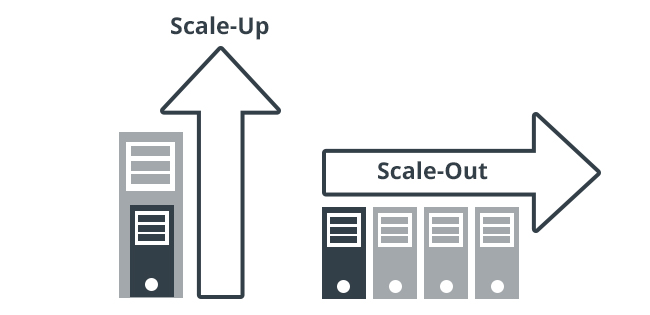
\includegraphics[width=0.7\textwidth]{resources/scales}
\caption[Skalierung]{Skalierung\protect\footnotemark}
\label{img:scales}
\end{figure}
\footnotetext{Skalierung: \url{https://magazin.kapilendo.de/den-supergau-verhindern-so-bereiten-sie-ihre-website-auf-einen-besucheransturm-vor/}, zugegriffen am 15. Januar 2017}

\subsubsection{\colorbox{green}{Vertikale Skalierung}}
%\subsubsection{Vertikale Skalierung}

Die vertikale Skalierung \textit{(scale-up)} strebt die qualitative Steigerung der Leistungsfähigkeit an, bei der die schon eingesetzten Ressourcen beispielsweise durch die Speichererweiterung oder CPU-Steigerung einfach verbessert werden.

\subsubsection{\colorbox{green}{Horizontale Skalierung}}
%\subsubsection{Horizontale Skalierung}

Die horizontale Skalierung \textit{(scale-out)}, im Gegensatz zur vertikalen Skalierung verteilt die Daten auf verschiedenen Knoten im großen Cluster, wobei die quantitative Steigerung der Leistungsfähigkeit angestrebt wird. Somit können mehrere weniger leistungsfähigere, nicht so teuere Rechner eingesetzt werden. Dadurch ist es möglich, sehr große horizontale Skalierbarkeit zu gewährleisten, da die Knoten somit nicht so stark, im Vergleich zur vertikalen Skalierung überlastet sind. 

\section{NoSQL-Datenbanken}
Im Vergleich zu den relationalen Datenbanken, die sich als eine strukturierte Sammlung von Tabellen (den Relationen) vorstellen, in welchen Datensätze abgespeichert sind, eignen sich NoSQL-Datenbanken zur unstrukturierter Daten, die einen nicht-relationalen Ansatz verfolgen. 

%Typische Beispiele für unstrukturierte Daten sind: Benutzer- und Sitzungsdaten, Chat-, Messaging- und Protokolldaten, Zeitreihendaten wie IoT- und Gerätedaten sowie große Objekte wie Videos und Bilder.\footnote{NSQL-Datenbanken: \url{http://de.basho.com/resources/nosql-databases/}, zugegriffen am 20. Dezember 2016}

\subsection{Was ist NoSQL?}
Der Begriff NoSQL steht nicht für 'kein SQL', sondern für 'nicht nur SQL' (Not only SQL). Das Ziel von NoSQL ist, relationale Datenbanken sinnvoll zu ergänzen, wo sie Defizite aufzeigen. Entstanden ist dieses Konzept in erster Linie als Antwort zur Unflexibilität, sowie zur relativ schwierigen Skalierbarkeit von klassischen Datenbanksystemen, bei denen die Daten nach einem stark strukturierten Modell gespeichert werden müssen.\footnote{MySQL vs. MongoDB: \url{http://www.computerwoche.de/a/datenbanksysteme-fuer-web-anwendungen-im-vergleich,2496589}, zugegriffen am 3. Januar 2016} Dokumentdatenbanken gruppieren die Daten in einem strukturierten Dokument, typischerweise in einer JSON-Datenstruktur. Auch \mongo, siehe dazu Abschnitt \ref{mongo} verfolgt diesen Ansatz und bietet darauf aufbauend eine reichhaltige Abfragesprache und Indexe auf einzelne Datenfelder. Die Möglichkeiten der Replikation und des Shardings zur stufenlosen und unkomplizierten Skalierung der Daten und Zugriffe macht \mongo\ auch für stark frequentierte Websites äußerst interessant.(\cite{Hollosi.2012}, Kapitel 14, Seite 435)

Beispiele für NoSQL-Datenbanken....:
\begin{multicols}{2}
\begin{itemize}
\item CouchDB
\item MongoDB
\item Redis
\item Google BigTable
\item Amazon Dynamo
\item Apache Cassandra
\item Hbase (ApacheHadoop)
\item Twitter Gizzard
\item weitere…
\end{itemize}
\end{multicols}
Jede NoSQL-Datenbanke verfolgt seine Ziele und welche sie genau verfolgen, beschreibt der Abschnitt \ref{categoryNoSQL}, in dem verschiedene Kategorien von NoSQL-Datenbanken vorgestellt werden.

\subsection{\colorbox{yellow}{Das CAP-Theorem}}\label{cap}
%\subsection{Das CAP-Theorem}\label{cap}

Im Jahr 2000 hielt Brewer\footnote{Eric A. Brewer ist ein Informatik-Professor an der University of California, Berkeley und einer der Erfinder der Suchmaschine Inktomi} die Keynote auf dem ACM Symposium on Principles of Distributed Computing (PODC)\footnote{PODC2000: \url{http://www.podc.org/podc2000/}, zugegriffen am 02.01.2017}, einer Konferenz über die Grundlagen der Datenverarbeitung in verteilten Systemen\footnote{In einem verteilten System im Bereich Datenverarbeitung werden gespeicherte Daten mehrfach über mindestens zwei verschiedene Server repliziert und miteinander synchronisiert, um die Verfügbarkeit der Daten zu erhöhen und die Zugriffszeiten der User zu verringern.} (Principles of Distributed Computing).  In seiner Keynote stellte Brewer sein \textbf{CAP}-Theorem vor, ein Ergebnis seiner Forschungen zu verteilten Systemen an der University of California \cite[S. 13]{Kurowski.2012}. Brewer's Theorem wurde im Jahr 2002 von Seth Gilbert und Nancy Lynch formal bewiesen.

\begin{figure}[H]
\centering
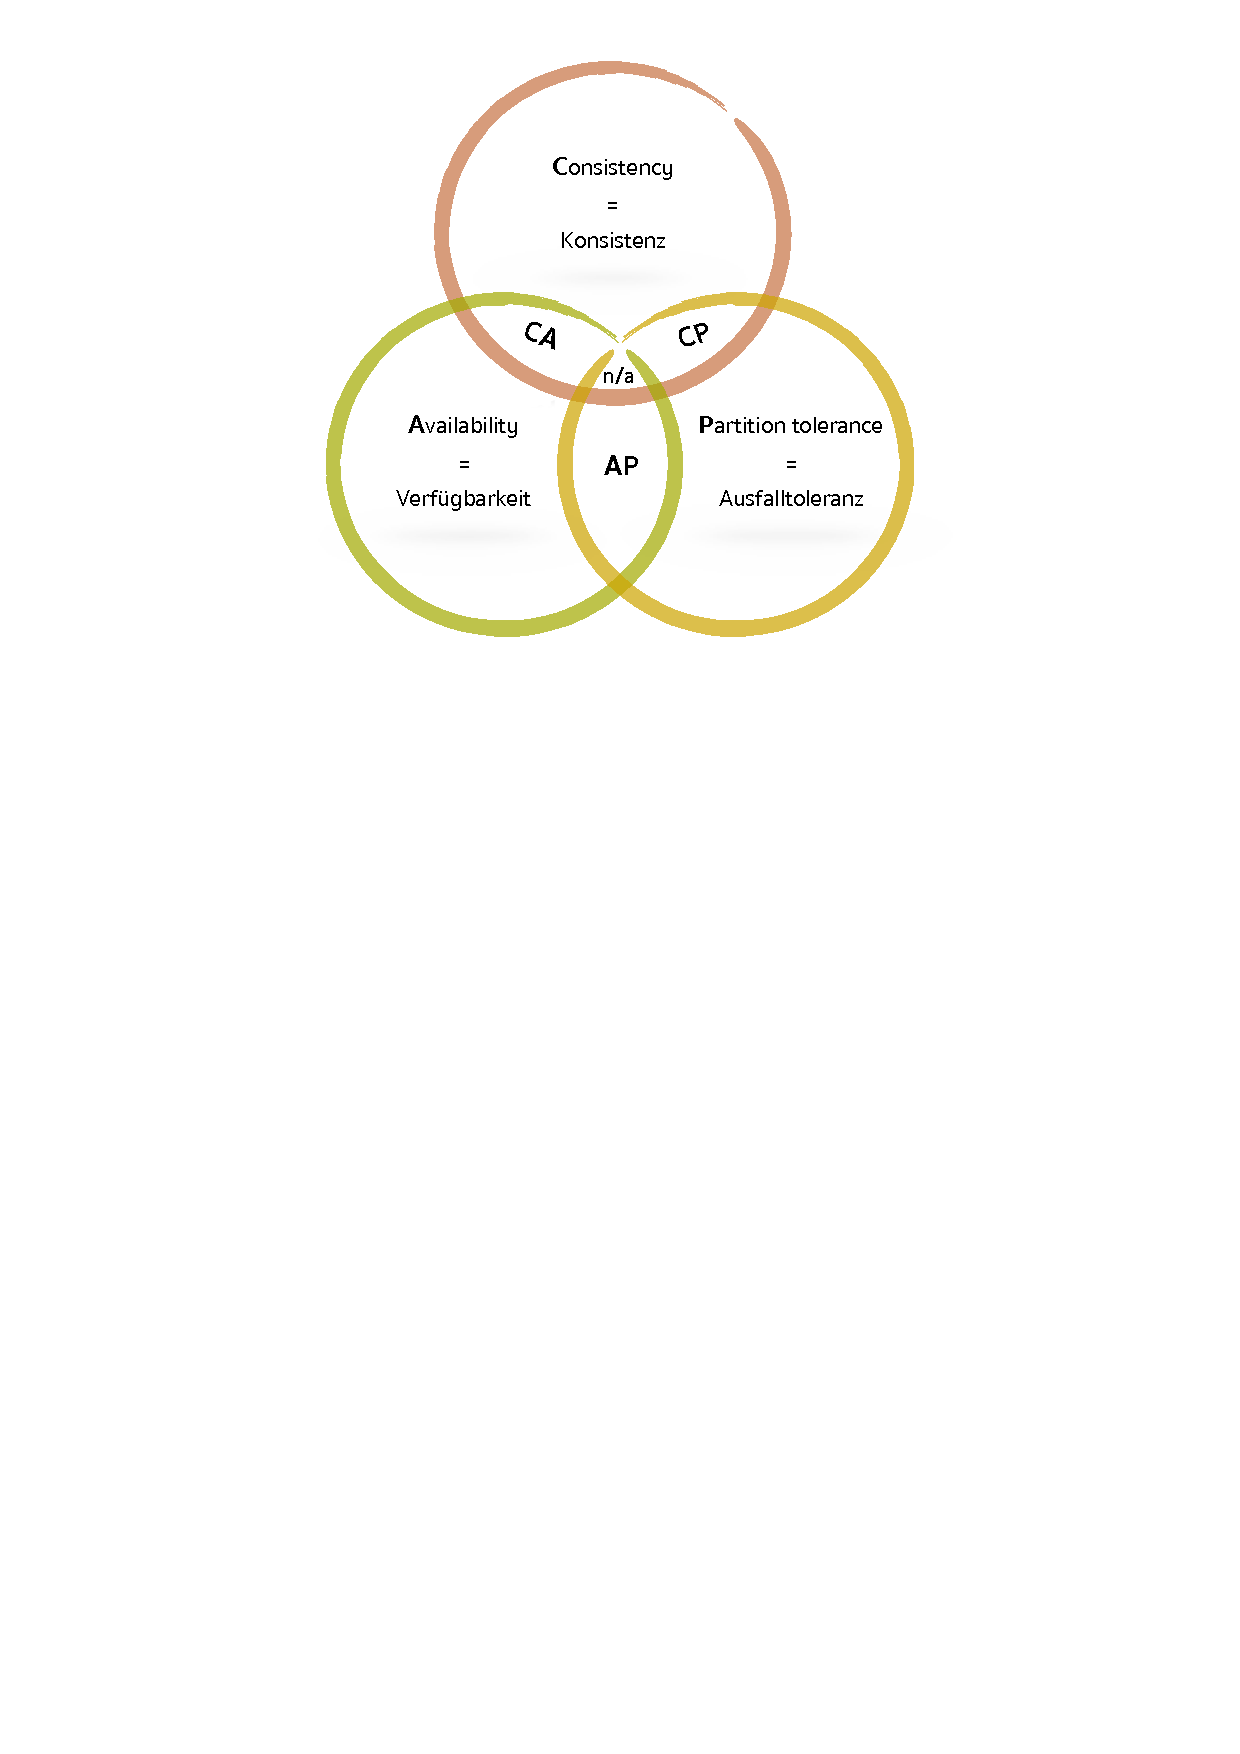
\includegraphics[trim = 0mm 189mm 0mm 9mm, clip, width=1.0\textwidth]{resources/myPictureForCAP}
\caption[\textbf{CAP}-Theorem]{Anforderungen an verteilte Systeme gemäß dem \textbf{CAP}-Theorem}
\label{img:cap}
\end{figure}

Das Akronym \textbf{CAP} steht für die englischsprachigen Begriffe  \Cap, \cAp\ und \caP\ und beschreiben die Anforderungen für die Skalierung an verteilte Systeme, die es zunächst näher zu erläutern gilt.

Was besagt eigentlich dieses \textbf{CAP}-Theorem? Das \textbf{CAP}-Theorem besagt, dass die verteilten Systeme, die mit großen Datenmengen zu tun haben, gleichzeitig die folgenden Anforderungen wie \Cap, \cAp\ und \caP\ nicht erfüllen können.
\begin{itemize}
\item \Cap: Die \textit{Konsistenz} der Daten in einem verteilten System wird im Prinzip genauso geschätzt wie im Abschnitt \ref{acid} die schon besprochene \Acid-Eigenschaft. Bedeutet, dass alle replizierenden Knoten aus einem großen Cluster über die gleichen Daten verfügen. Falls ein Wert auf einem Knoten durch eine Transaktion per Schreiboperation geändert wird, muss der aktualisierte Wert auf Anfrage mit der Leseoperation von anderen Knoten zurückgeliefert werden können. Die Transaktion selbst ist eine atomare\footnote{Eine atomare Transaktion bedeutet, dass sie entweder ganz oder gar nicht ausgeführt wird. Falls eine atomare Transaktion abgebrochen wird, werden alle im Laufe der Transaktion schon durchgeführte Änderungen rückgängig gemacht.} Einheit in der Datenbank.

\item \cAp: Die \textit{Hochverfügbarkeit} ist die weitere Anforderung, die besagt, dass immer alle gesendeten Anfragen durch User ans System beantwortet werden müssen und mit einer akzeptablen Reaktionszeit.
\item \caP: Die \textit{Partitions- oder Ausfalltoleranz} bedeutet, dass der Ausfall eines Knoten bzw. eines Servers aus einem Cluster das verteilte System nicht beeinträchtigt und es fehlerfrei weiter funktioniert. Falls einzelne Knoten in so einem System ausfallen, wird deren Ausfall von den verbleibenden Knoten aus dem Cluster kompensiert, um die Funktionsfähigkeit des Gesamtsystems aufrecht zu halten.

\end{itemize}

Die graphische Darstellung für das Brewer's \textbf{CAP}-Theorem ist aus der Abbildung \ref{img:cap} zu entnehmen. Wie die Abbildung \ref{img:cap} erkennen lässt, können in einem verteilten System gleichzeitig und vollständig nur zwei dieser drei Anforderungen  \Cap, \cAp, \caP\ erfüllt sein. Konkret aus der Praxis bedeutet das, dass es für eine hohe Verfügbarkeit und Partitions- oder Ausfalltoleranz notwendig ist, die Anforderungen an die Konsistenz zu lockern \cite[S. 31]{Edlich.2011}.

Die Anforderungen in Paaren klassifizieren gemäß dem \textbf{CAP}-Theorem bestimmte Datenbanktechnologien. Für jede Anwendung muss daher individuell entschieden werden, ob sie als ein \textbf{CA-}, \textbf{CP-} oder \textbf{AP-}System zu realisieren ist.
\begin{itemize}
\item \textbf{CA} (\textbf{C}onsistency und \textbf{A}vailability): Die klassischen relationalen Datenbankmanagementsysteme (RDBMS) wie Oracle, DB2 etc. fallen in \textbf{CA}-Kategorie, die vor allem \Cap\ und \cAp\ aller Knoten in einem Cluster hinzielt. Hierbei werden die Daten nach dem \textbf{ACID}-Prinzip verwaltet. Die relationalen Datenbanken sind für Ein-Server-Hardware konzipiert und vertikal skalierbar. Das bedeutet, dass solche Systeme mit hochverfügbaren Servern betrieben werden und \caP\  nicht unbedingt in Frage kommt.

\begin{itemize}
\item keine Partitionstoleranz
\item (Relationale) Datenbank ermöglicht verteilte Transaktionen zur Konsistenzwahrung
\item Voraussetzung: funktionierendes Netzwerk (kein Nachrichtenverlust)
\item URL: \url{http://dbs.uni-leipzig.de/file/NoSQL_SS14_01_Intro.pdf}
\end{itemize}

\item \textbf{CP} (\textbf{C}onsistency und \textbf{P}artition tolerance): Ein gutes Beispiel für die Anwendungen, die zu der \textbf{CP-}Kategorie zu zuordnen sind, sind Banking-Anwendungen. Für solche Anwendungen ist es wichtig, dass die Transaktionen zuverlässig durchgeführt werden und der mögliche Ausfall eines Knotens sichergestellt wird.

\begin{itemize}
\item keine Verfügbarkeit
\item im Falle von Netzwerkpartitionierung werden Transaktionen blockiert
\item Vermeidung möglicher Konflikte bei Merge, dadurch Sicherstellung der Konsistenz
\item URL: \url{http://dbs.uni-leipzig.de/file/NoSQL_SS14_01_Intro.pdf}
\end{itemize}

\item \textbf{AP} (\textbf{A}vailability und \textbf{P}artition tolerance): Für die Anwendungen, die in die \textbf{AP-}Kategorie fallen, rückt die Anforderung \Cap\ in den Hintergrund. Beispiele für solche Anwendungen sind die Social-Media-Sites wie Twitter\footnote{Twitter: \url{https://twitter.com/}} oder Facebook\footnote{Facebook: \url{https://www.facebook.com/}}, da die Hauptidee der Anwendung dadurch nicht verfällt, wenn zum gleichen Zeitpunkt die replizierten Knoten nicht über die gleiche Datenstruktur verfügen. 
\end{itemize}

\begin{itemize}
\item keine Konsistenz
\item Writes stets möglich auch wenn keine Kommunikation mit anderen Knoten möglich
(z.B. Synchronisation)
\item Notwendigkeit der Auflösung inkonsistenter Daten, d.h. verschiedene Versionen des
selben Datums an verschiedenen Knoten
\item URL: \url{http://dbs.uni-leipzig.de/file/NoSQL_SS14_01_Intro.pdf}
\end{itemize}

\subsection{\colorbox{yellow}{BASE}}
%\subsection{BASE}
\textbf{BASE} steht für \BAse, \baSe, \basE\ und beschreibt den Gegenteil zu den strengen \textbf{ACID}-Kriterien aus dem Teilabschnitt \ref{acid}. \textbf{BASE} ist wie \textbf{CAP}-Theorem (Teilabschnitt \ref{cap}) auch für verteilte Datenbanksysteme formuliert, für die die \textit{Konsistenz} nicht mehr im Vordergrund steht, sondern die \textit{Verfügbarkeit} eines Systems. Bei solchen Systemen, die nach dem \textbf{BASE}-Prinzip gestaltet sind, ist eher wichtig, dass für alle Clients das System ständig verfügbar ist. Die Clients müssen nicht unbedingt zu dem gleichen Zeitpunkt die gleichen Daten sehen.

\subsection{\colorbox{red}{Arten von NoSQL-Datenbanken}}\label{categoryNoSQL}
\colorbox{red}{Eigene Graphen als Abbildungen verwenden, diese sind nur als Beispiel drin......!}
%\subsection{Arten von NoSQL-Datenbanken}\label{categoryNoSQL}
Der folgende Abschnitt stellt insgesamt vier Kategorien von NoSQL-Datenbanken dar, wie in der Abbildung \ref{img:nosqlgroups} zu sehen ist.
\begin{figure}[H]
\centering
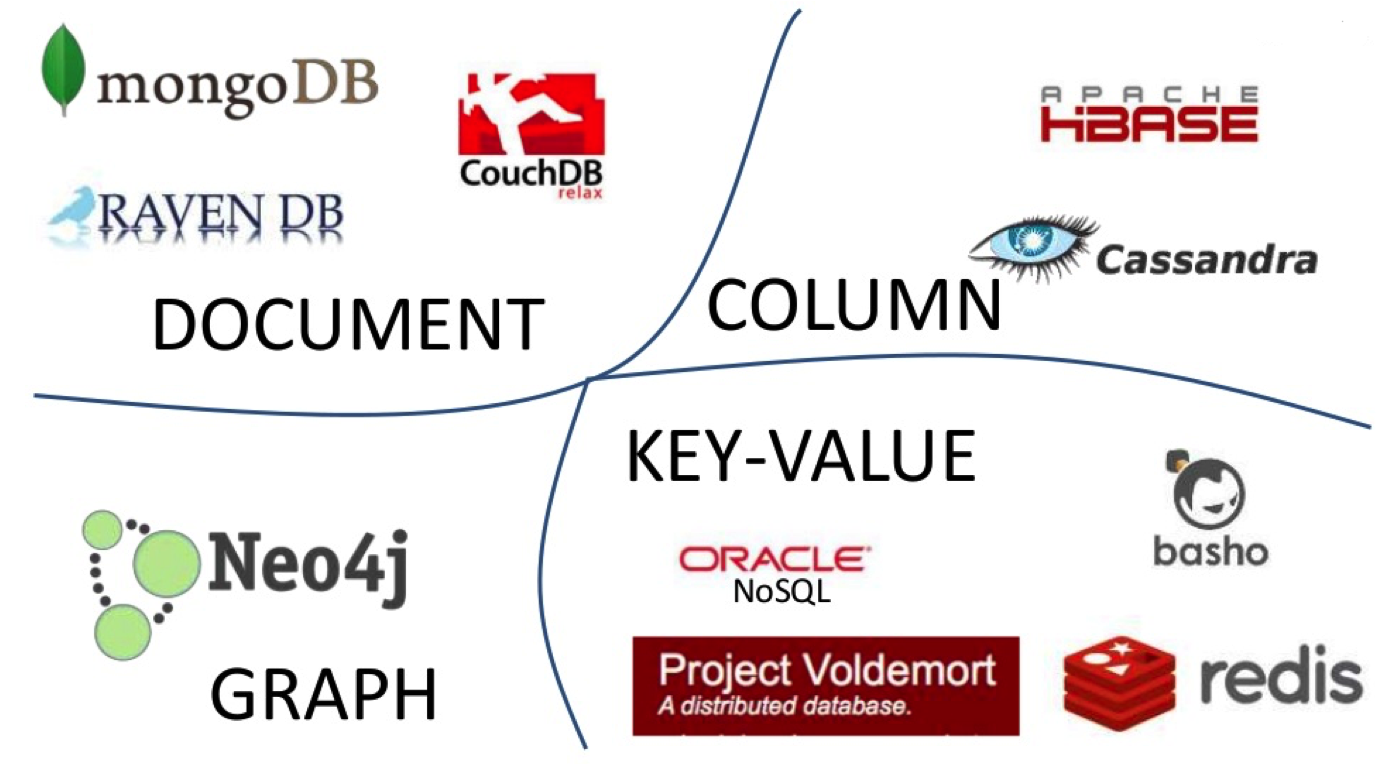
\includegraphics[width=0.5\textwidth]{resources/nosqlgroups}
\caption[NoSQL-Datenbanken]{NoSQL-Datenbanken, verteilt in vier Gruppen\protect\footnotemark}
\label{img:nosqlgroups}
\end{figure}
\footnotetext{NoSQL-Datenbanken: \url{http://bigdata-blog.com/key-value-database}, zugegriffen am 17. Januar 2017}
Die \mongo\ wird im Abschnitt \ref{mongo} detailliert beschrieben. BlaBlaBla
\subsubsection{Key-Value-Datenbanken}

Eine Key-Value-Datenbank \textit{(Key-Value Store)} ist eine Datenbank, in der die Daten in Form von Schlüssel-Werte-Paaren abgespeichert werden. Der Schlüssel verweist dabei auf einen eindeutigen (meist in Binär- oder Zeichenketten-Format vorliegenden) Wert\footnote{NoSQL: Key-Value-Datenbank Redis im Überblick: \url{https://www.heise.de/developer/artikel/NoSQL-Key-Value-Datenbank-Redis-im-Ueberblick-1233843.html}, zugegriffen am 17. Januar 2017}. Value kann oft beliebiger Datentyp wie Arrays, Dokumente, Objekte, Bytes etc. sein. Siehe dazu die Abbildung \ref{img:kvdb} mit einem Beispiel:

\begin{figure}[H]
\centering
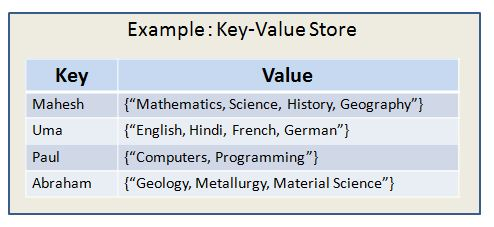
\includegraphics[width=0.6\textwidth]{resources/kvdb}
\caption[NoSQL: A Silver Bullet for handling Big Data?]{Key-Value-Datenbank als Beispiel\protect\footnotemark}
\label{img:kvdb}
\end{figure}
\footnotetext{NoSQL: A Silver Bullet for handling Big Data?: \url{https://www.linkedin.com/pulse/nosql-silver-bullet-handling-big-data-shashank-dhaneshwar}, zugegriffen am 17. Januar 2017}

%Wie der Überschrift vermuten lässt, sind die Datensätze mit Key-Value-Paaren zu verwalten. 

\subsubsection{Spaltenorientierte Datenbanken}

In einer spaltenorientierten Datenbank \textit{(Column Store)}, wie der Name vermuten lässt, werden die Datensätze spalten- statt zeilenweise abgespeichert. Durch die spaltenorientierte Abspeicherung der Daten wird der Lesezugriff stark beschleunigt, da keine unnötigen Informationen mehr gelesen werden, stattdessen nur diejenigen, die wirklich benötigt wurden. Dadurch wird der Schreibprozess aber erschwert, falls die schreibenden Daten aus mehreren Spalten bestehen werden, auf die entsprechend zugegriffen werden muss. Der Schreibprozess wird sich in diesem Fall etwas verlangsamen.

\colorbox{red}{Abbildung==?????}

\subsubsection{Graphen-Datenbanken}
Eine Graphen-Datenbank \textit{(Graph database)} ist weitere Kategorie aus der NoSQL Gruppe, in der die Daten anhand eines Graphen dargestellt und abgespeichert werden.

\begin{figure}[H]
\centering
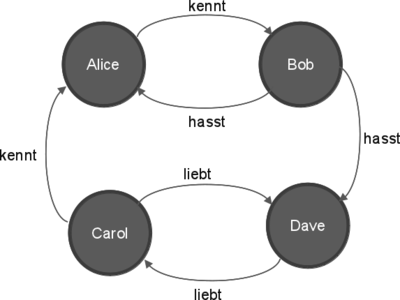
\includegraphics[width=0.5\textwidth]{resources/gdb}
\caption[Beispiel für die Darstellung der Daten in einer Graphen-Datenbank]{Beispiel für die Darstellung der Daten in einer Graphen-Datenbank\protect\footnotemark}
\label{img:gdb}
\end{figure}
\footnotetext{Beispiel für die Darstellung der Daten in einer Graphen-Datenbank: \url{https://de.wikipedia.org/wiki/Graphdatenbank}, zugegriffen am 17. Januar 2017}

Wie der Abbildung \ref{img:gdb} zu entnehmen ist, bestehen Graphen grundsätzlich aus Knoten \textit{(Node)} und Kanten \textit{(Edge)}. Dabei stellen die Kanten die Verbindungen zwischen den einzelnen Knoten dar.
%\subsubsection{Objektdatenbanken }
%\textit{(Object database)}

%\begin{tikzpicture}[remember picture,overlay]
%\node[anchor=east,inner sep=0pt] at (current page text area.east|-0,6cm) %{
\includegraphics[height=4cm]{resources/mongoDBlogo}};
%\end{tikzpicture}
\subsubsection{Dokumentenorientierte Datenbanken}

Eine Datenbank, in der die Daten in Form von Dokumenten abgespeichert werden, ist als eine dokumentenorientierte Datenbank \textit{(Document Store)} zu definieren. In diesem Zusammenhang ist ein Dokument als eine Zusammenstellung bestimmter Daten zu verstehen, das mit einem eindeutigen Identifikator angesprochen werden kann. Da die Daten in der dokumentenorientierte Datenbank nicht in Form von Tabellen, sondern in Form von Dokumenten abgespeichert werden, ergibt sich daraus keinen Strukturzwang. Als Beispiel ist aus der Abbildung \ref{img:dodb} zwei Dokumente im \textbf{JSON}-Format zu entnehmen, die sich voneinander gänzlich unterscheiden.
\begin{figure}[H]
\centering
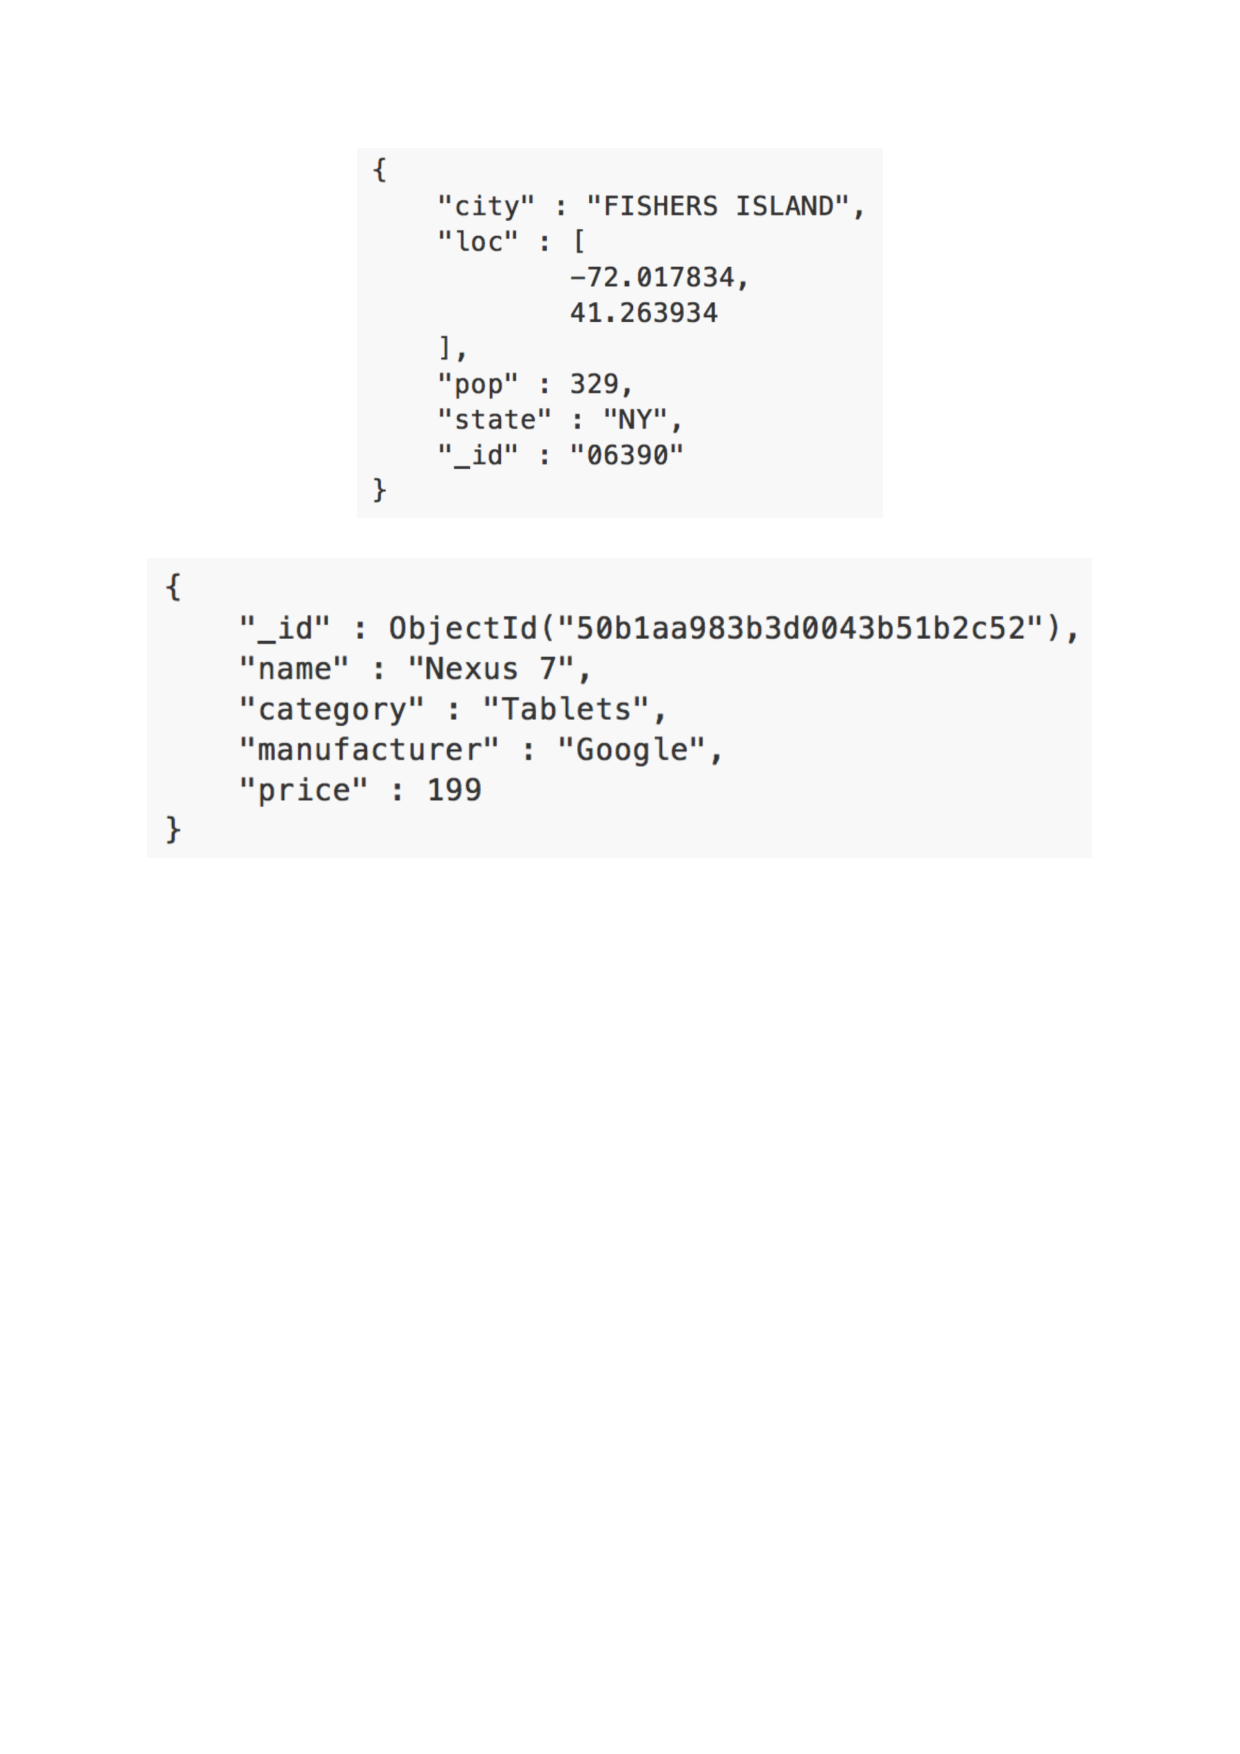
\includegraphics[trim = 0mm 150mm 0mm 20mm, clip, width=0.7\textwidth]{resources/dodb}
\caption[Zwei Dokumente im JSON Format]{Zwei Dokumente im JSON Format}
\label{img:dodb}
\end{figure}
Möchte man ein bestimmtes Dokument erweitern, so kann man es einfach tun, da eine dokumentenorientierte Datenbank strukturfrei ist. Weitere Datenformate sind beispielsweise YAML\footnote{YAML: \url{http://www.yaml.org/start.html}} (angelehnt an XML) oder XML\footnote{XML: \url{https://www.xml.com/}} selbst.
%Die dokumentenorientierte Datenbank hat somit keinen Strukturzwang, da die Datensätze in einzelne voneinander unabhängige Dokumente gespeichert werden. Ein Beispiel dazu ist aus der der Abbildung XX zu entnehmen.
%Siehe Artikel \url{http://pi.informatik.uni-siegen.de/Mitarbeiter/mrindt/Lehre/Seminare/NoSQL/einreichungen/NOSQLTEC-2015_paper_9.pdf}
%siehe \cite[S. 5-8]{Edlich.2011}

\section{MongoDB}\label{mongo}
\mongo\ ist eine  schemalose, dokumentenorientierte Open-Source-Datenbank und gehört somit zu einer der im Teilabschnitt \ref{categoryNoSQL} besprochenen Arten von NoSQL-Datenbanken. Der Name stammt von dem englischen Begriff \textit{hu}MONGO\textit{us}, ins Deutsche als \textit{gigantisch} oder \textit{riesig} übersetzen lässt. Die genannte NoSQL-Datenbank macht mit seinem effizienten dokumentenorientierten Ansatz, einfacher Skalierbarkeit und hoher Flexibilität dem bewährten MySQL\footnote{MySQL: \url{https://www.mysql.com}}-System zunehmend Konkurrenz.\footnote{MySQL vs. MongoDB: \url{http://www.computerwoche.de/a/datenbanksysteme-fuer-web-anwendungen-im-vergleich,2496589}, zugegriffen am 19. Januar 2017} 

Die Unterschiede zu den Konzepten der relationalen und nicht-relationalen Datenbanken konkret von \mongo\ stellt die Tabelle \ref{table:concepts} dar.

\rowcolors{1}{white}{lightgray}
\newcommand*{\head}[1]{\textbf{#1}}%

\begin{table}[H]
\centering
\begin{tabular}{ccc}
  \toprule[1.5pt]
  \head{Relational} & \head{\mongo}\\
  \midrule
  \rmfamily Database & \rmfamily Database\\
    \rmfamily Table & \rmfamily Collection\\ 
      \rmfamily Row & \rmfamily Document\\ 
        \rmfamily Index & \rmfamily Index\\ 
          \rmfamily Join & \rmfamily Lookup\\ 
            \rmfamily Foreign Key & \rmfamily Reference\\ 
              \rmfamily Multi-table transaction & \rmfamily Single document transaction\\ 
  \bottomrule[1.5pt]
\end{tabular}
\caption{Konzepte}
\label{table:concepts}
\end{table}

\subsection{\colorbox{red}{Datensätze in Form von Dokumenten}}
%\subsection{Datensätze in Form von Dokumenten}
Die NoSQL-Datenbank \mongo\ verwendet für die Dokumentenspeicherung und den Datenaustausch das sogenannte \textbf{BSON}\footnote{BJSON: \url{http://www.bjson.org}}-Format, das eine binäre Darstellung von \textbf{JSON}-ähnlichen Dokumenten bietet.
%speichert Daten in Form von Dokumenten im \textbf{BJSON}\footnote{BSON: \url{http://www.bjson.org}}-Format.
Die Dokumente selbst werden von \mongo\ in sogenannten Kollektionen \textit{(Collections)} gespeichert. Wie es schon aus dem Abschnitt \ref{categoryNoSQL} bekannt ist, kann jedes Dokument eine beliebige Anzahl an Feldern besitzen, unabhängig voneinander. 

Zudem dürfen Dokumente auch innerhalb eines Dokuments gespeichert werden\footnote{Einführung in MongoDB: \url{https://www.iks-gmbh.com/assets/downloads/Einfuehrung-in-MongoDB-iks.pdf}, zugegriffen am 19. Januar 2017}. Die Speicherung von Daten in Form von Dokumenten bietet den Vorteil, das sowohl strukturierte, als auch semi-strukturierte und polymorphe Daten gespeichert werden können. Dokumente, die jedoch das gleiche oder ein ähnliches Format haben, sollten zu einer Kollektion \textit{(Collection)} zusammengefasst werden\footnote{MongoDB: \url{http://www.moretechnology.de/mongodb-eine-dokumentenorientierte-datenbank/}, zugegriffen am 21. Januar 2017}.

\subsection{\colorbox{red}{Die Nexus Architektur}}
%\subsection{Die Nexus Architektur}

Die MongoDB konzentriert sich auf die Kombination blabla


Zu den wichtigsten Eigenschaften, die für einen Einsatz von \mongo\ sprechen, gehören:
\begin{itemize}
\item Hochverfügbarkeit: Auch bei Ausfall einer Datenbankinstanz soll die Applikation weiterhin verfügbar bleiben, d. h. nahtlos – ohne manuellen Eingriff – müssen redundante Instanzen bei einem Ausfall einspringen
\item Skalierbarkeit: Mit transparentem Sharding, siehe Teilabschnitt \ref{sharding} – einem Verfahren zur horizontalen Skalierung – kann die Infrastruktur vergleichsweise einfach wachsenden Anforderungen angepasst werden
\item Performanz: Vom Ansatz her haben dokumentenorientierte DBMS hier einen Vorteil, weil die Daten nicht erst aus mehreren Tabellen zusammengeführt werden\footnote{MongoDB Eigenschaften: \url{https://entwickler.de/online/datenbanken/mongodb-erfolgreich-ein-dokumentenorientiertes-datenbanksystem-einfuehren-115079.html}, zugegriffen am 12. Dezember 2016}
\end{itemize}

Die Vorteile relationaler und NoSQL-Datenbanken sind aus der Abbildung \ref{img:architektur} zu entnehmen.
\begin{figure}[H]
\centering
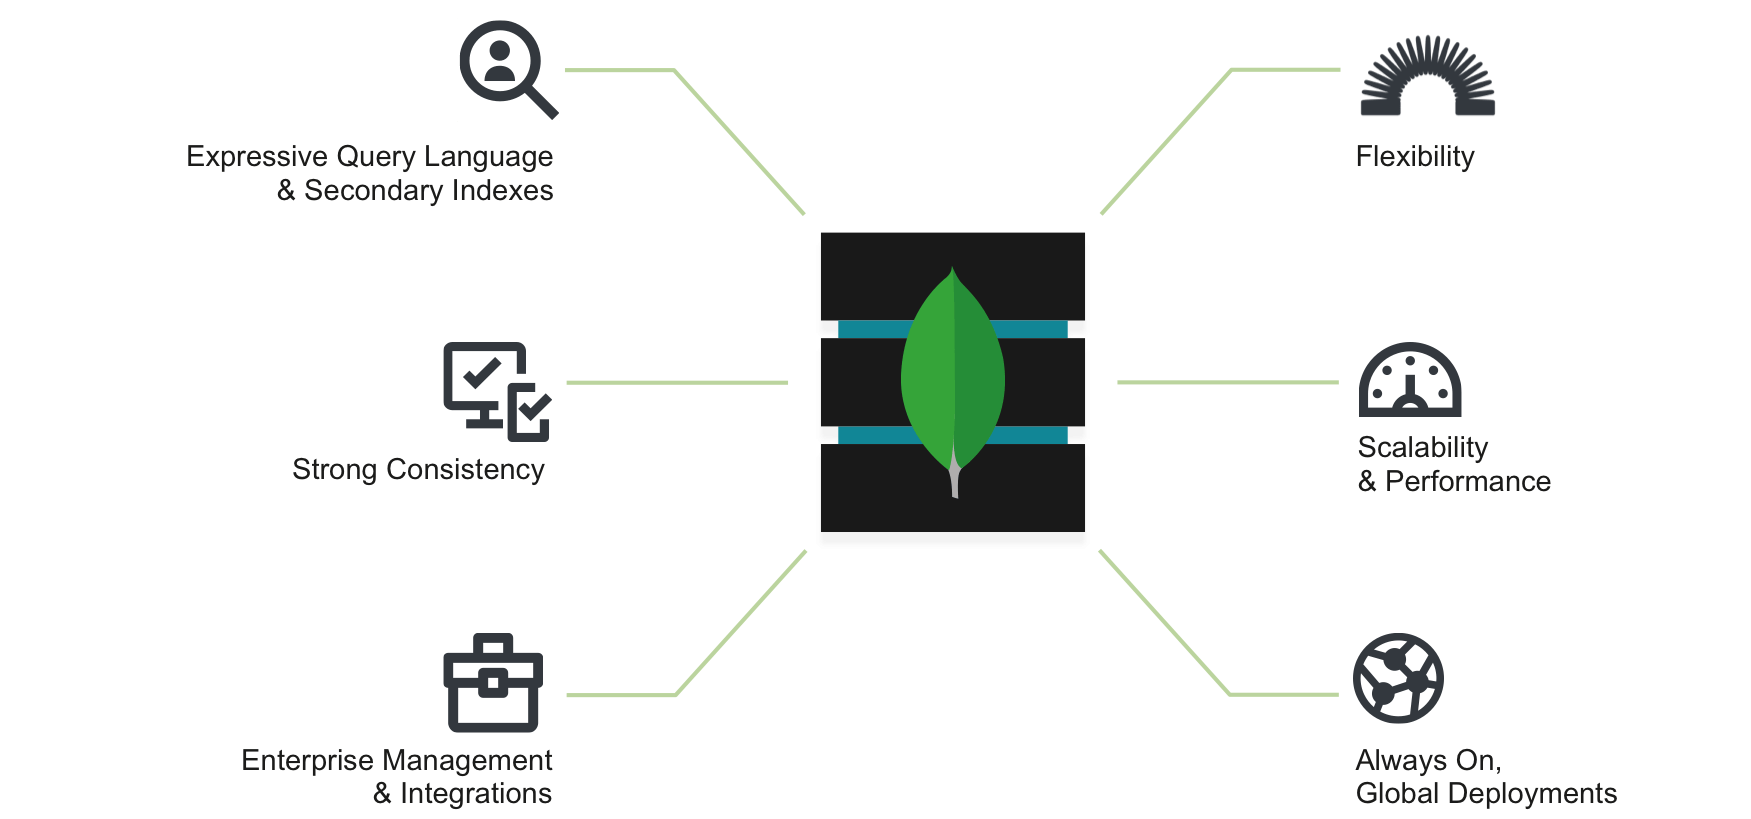
\includegraphics[width=1.0\textwidth]{resources/architecture}
\caption[MongoDB Architektur]{MongoDB Architektur\protect\footnotemark}
\label{img:architektur}
\end{figure}
\footnotetext{MongoDB Architektur: \url{https://www.mongodb.com/mongodb-architecture}, zugegriffen am 28. Januar 2016}

\subsection{CRUD = IFUR}\label{ifur}
\textit{\textbf{CRUD}}-Operationen heißen in MongoDB \textit{\textbf{I}nsert}, \textit{\textbf{Fi}nd}, \textit{\textbf{U}pdate} und \textit{\textbf{R}emove}.

Bei \mongo\ ist es nicht einmal notwendig, eine Datenbank oder eine Collection zu definieren, bevor etwas gespeichert werden wird. Datenbanken und Collections werden zur Laufzeit beim ersten Einfügen eines Dokuments von MongoDB erzeugt.

\subsubsection{Create/Insert}
blablablabla
\begin{listingsboxShell}[label={lst:insert}]{myshell}{Dokument(e) speichern}
> db.collection.insert(..)
> db.collection.insertMany(..)
> db.collection.insertOne(..)
\end{listingsboxShell}
\subsubsection{Read/Find}
blablablabla
\begin{listingsboxShell}[label={lst:find}]{myshell}{Dokument(e) finden}
> db.collection.find(..)
> db.collection.findOne(..)
> db.collection.findOneAndDelete(..) etc.
\end{listingsboxShell}
\subsubsection{Update/Update}
blablablabla
\begin{listingsboxShell}[label={lst:update}]{myshell}{Dokument(e) aktualisieren}
> db.collection.update(..)
> db.collection.updateMany(..)
> db.collection.updateOne(..)
\end{listingsboxShell}
\subsubsection{Delete/Remove}
blablablabla
\begin{listingsboxShell}[label={lst:remove}]{myshell}{Dokument(e) löschen}
> db.collection.remove(..)
\end{listingsboxShell}

\subsection{Indizes}
Indizes in MongoDB werden als Binär-Baum\footnote{Binär-Baum: \url{http://www.hs-augsburg.de/mebib/emiel/entw_inf/lernprogramme/baeume/gdi_kap_4_1.html}, zugegriffen am 23. Dezember 2016} in einer vordefinierten Sortierreihenfolge abgelegt, siehe Abbildung \ref{img:IndexesInMongoDBAreB-Trees}
\begin{figure}[H]
\centering
	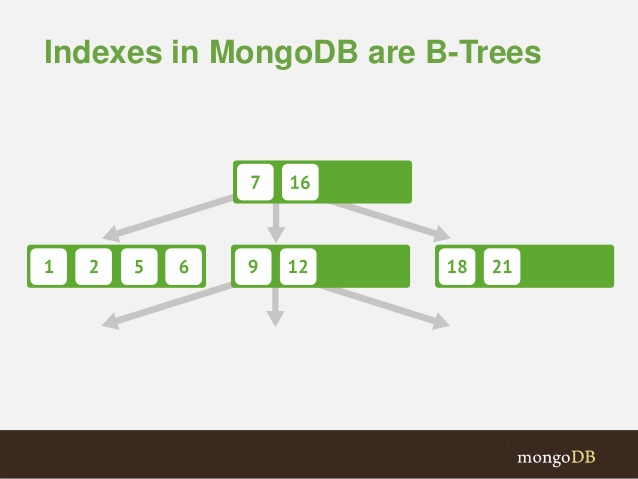
\includegraphics[width=0.7\textwidth]{resources/indexingBtree}
\caption[Indizes in \mongo\ als Binär-Baum]{Indizes in \mongo\ als Binär-Baum\protect\footnotemark}
\label{img:IndexesInMongoDBAreB-Trees}
\end{figure}
\footnotetext{Indizes in MongoDB als Binär-Baum: \url{http://www.slideshare.net/mongodb/indexing-strategies-to-help-you-scale}, zugegriffen am 23. Dezember 2016}

Der Index wird beim Erstellen, Updaten und Löschen eines Dokumentes auch aktualisiert. Zu viele Indizes machen schreib Operationen langsam und die Größe der Indizes steigt an, deswegen sollte ein Index nur auf Felder zeigen, auf die auch Query-Operationen angewendet werden. Beim Anlegen der Indizes ist die Sortierreihenfolge zu gunsten einer schnelleren Suche wichtig, da sie schon vorsortiert vorliegen und nicht erst bei der Liveabfrage sortiert werden müssen.\footnote{Indizes: \url{http://wikis.gm.fh-koeln.de/wiki_db/MongoDB/Indizes}, aufgerufen am 24. Dezember 2016}

Es gibt drei Möglichkeiten der Sortierung:

\begin{itemize}
\item Aufsteigend(1),
\item Absteigend (-1),
\item geospatial (2d).
\end{itemize}

Index hilft, Datenbanken zu optimieren. Die nachfolgende \autoref{img:EfficiencyofIndexUse} demonstriert

Neben dem obligatorischen Primär-Index auf dem Feld \_id, das in jedem Dokument existieren und pro Collection eindeutig sein muss, können Sie in MongoDB bis zu 63 weitere Sekundär-Indizes pro Collection anlegen, um Suchanfragen zu beschleunigen. Ein Sekundär-Index kann auf einem einzelnen Feld oder einer Gruppe von Feldern angelegt werden.%\footnote{Indizes: \url{https://www.informatik-aktuell.de/betrieb/datenbanken/mongodb-fuer-software-entwickler.html}}

Which optimization will typically have the greatest impact on the performance of a database?\newline
Adding appropriate indexes on large collections so that only a small percentage of queries need to scan the collection.

\subsubsection{Creating Indexes}
blabla

\begin{listingsboxShell}[label={lst:X}]{myshell}{Mongo-Shell: Something else}
> db.students.createIndex();
\end{listingsboxShell}

blabla

\begin{listingsboxShell}[label={lst:X}]{myshell}{Mongo-Shell: Something else}
> db.students.explain().find();
\end{listingsboxShell}

Quiz: Please provide the mongo shell command to add an index to a collection named students, having the index key be class, student\_name.
Neither will go in the "-1" direction..

\begin{listingsboxShell}[label={lst:X}]{myshell}{Something else}
> db.students.createIndex({student\_name:1, class:1});
\end{listingsboxShell}

\begin{listingsboxShell}[label={lst:X}]{myshell}{Mongo-Shell: Something else}
> db.students.dropIndex({student_name:1});
\end{listingsboxShell}

\subsubsection{Multikey Indexes}
blabla
\subsubsection{Index Creation Option, Unique}
für jedes attribut kann man Unique definieren, d.h. doppelte Werte dürfen nicht vorkommen\newline\newline

\begin{listingsboxShell}[label={lst:X}]{myshell}{Mongo-Shell: Something else}
> db.students.createIndex({student_id : test}, {unique:true});
\end{listingsboxShell}

Please provide the mongo shell command to create a unique index on student\_id, class\_id, ascending for the collection students.

\begin{listingsboxShell}[label={lst:X}]{myshell}{Mongo-Shell: Something else}
> db.students.createIndex({student_id:1, class_id:1}, {unique:true});
\end{listingsboxShell}

\subsubsection{Index Creation, Sparse}

Im Fall, wenn ein Attribut nicht in allen Dokumenten vorkommt, aber für dieses ein Unique Index definiert werden soll, muss Folgendes verwendet werden:

\begin{listingsboxShell}[label={lst:X}]{myshell}{Something else}
> db.students.createIndex({cell:1}, {unique:true, sparse:true});
\end{listingsboxShell}

blabla, siehe den Shellbefehl, blabla

\begin{listingsboxShell}[label={lst:X}]{myshell}{Something else}
> db.students.createIndex({student_id:1, class_id:1}, {unique:true});
\end{listingsboxShell}
siehe Codeauszug

\subsection{Aggregation Framework}\label{aggr}

Seit der Version 3.2 der dokumentenorientierten NoSQL-Datenbank \textbf{MongoDB}, die am 8. Dezember 2015 erschienen ist, ist \textit{Aggregation Framework}  mit zwei grundlegenden Features ergänzt worden, wie \textit{Fetch Joins} und \textit{Schema-Validierung}. Bislang waren die \textit{(Collections)} völlig isoliert voneinander, was die \textbf{CRUD}-Operationen (Teilabschnitt \ref{ifur}) erschwert hat. Mit \textit{Joins} ist es möglich geworden, Dokumente aus anderen \textit{(Collections)} mitzuladen.
\colorbox{red}{Über Schema-Validierung noch schreiben...}

\colorbox{red}{Ein Beispiel für Joins dazu hinzufügen, in dem ein eingebettetes Dokument gezeigt wird...!}

How good is it? Mapping between SQL and Aggregation
Um die Nutzung der Aggregation Framework in MongoDB zu ermöglichen, stellt MongoDB Java Driver zur Verfügung.  

\subsection{Horizontale Skalierung (Sharding)}
Um eine kostengünstige Lösung für eine Steigerung der Leistung von Systemen zu ermöglichen, ermöglicht das Datenbanksystem von \mongo\  eine horizontale Skalierung, die allgemein im Teilabschnitt \ref{scale} schon diskutiert ist. Die horizontale Verteilung der Daten erfolgt bei \mongo\ auf Ebene der \textit{Collections}, siehe Abbildung \ref{img:sharding}, mithilfe von sogenannten \textit{Sharding-Keys}. Die \textit{Sharding-Keys} dienen dazu, um später Zugriffe auf einzelne Dokumente zu ermöglichen.
\begin{figure}[H]
\centering
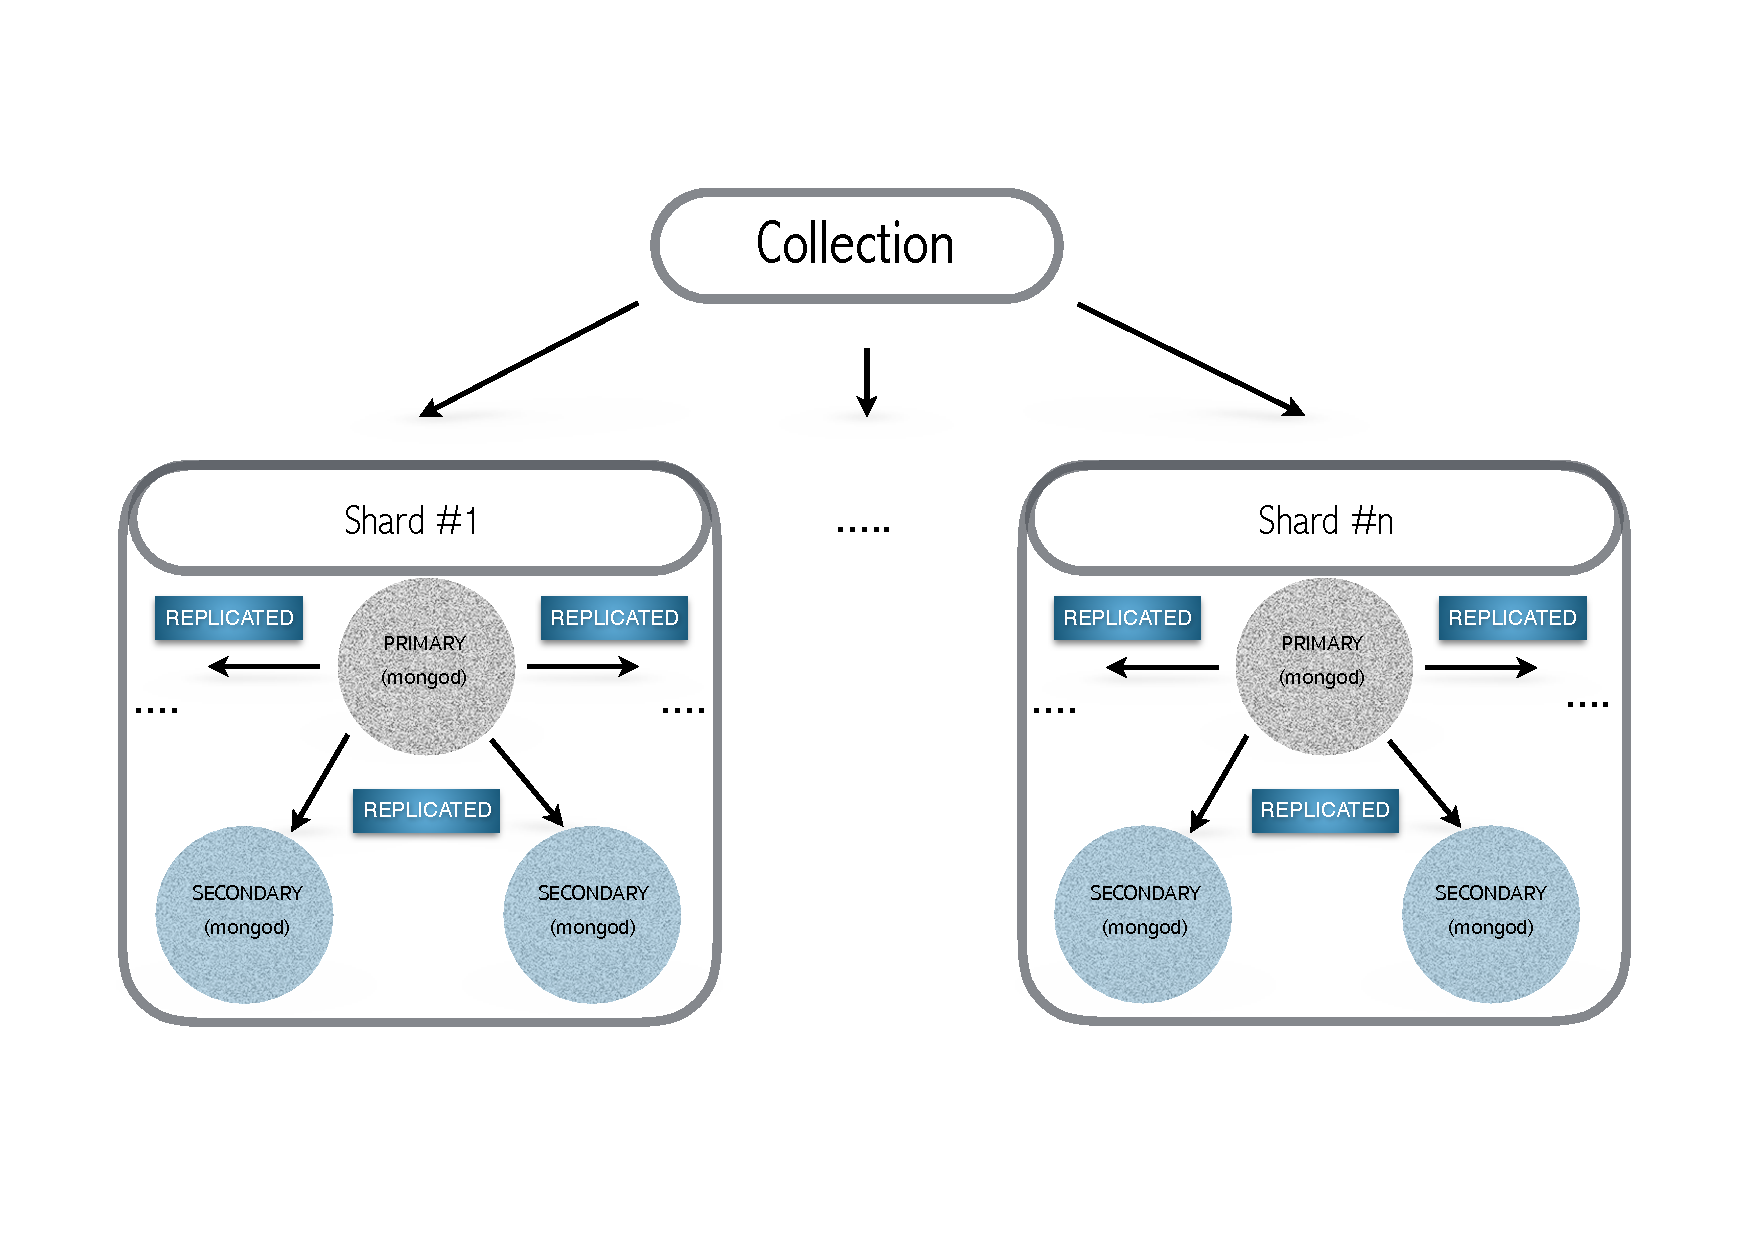
\includegraphics[trim = 0mm 35mm 0mm 30mm, clip, width=1.0\textwidth]{resources/replicaSet/sharding}
\caption[Ein Beispiel für Verteilung einer \textit{Collection} auf mehreren \textit{Shards}]{Ein Beispiel für Verteilung einer \textit{Collection} auf mehreren \textit{Shards}}
\label{img:sharding}
\end{figure}
Die Aufteilung der \textit{Collections} erfolgt in Blöcken, auch als \textit{Chunks} genannt. Ein \textit{Chunk} ist ein Teil einer bestimmten \textit{Collection}. Gespeichert werden \textit{Chunks} auf Servern, die in diesem Zusammenhang als \textit{Shards} bezeichnet werden. Was es unter \textit{Shards} zu verstehen ist, erläutert der Teilabschnitt \ref{replication} zur Replikation.

Um die Aufteilung der \textit{Collections} in \textit{Chunks} auf \textit{Shards} realisieren zu können, verwendet \mongo\ folgende Komponenten:
\begin{itemize}
\item \textit{shards:} Die \textit{Shards} enthalten letztendlich die Daten. In einer \textit{Shard} ist es möglich, Replikationsgruppen zu verwenden, näher dazu im Teilabschnitt \ref{replication}.
\item \textit{mongos:} \textit{mongos} gilt als ein \textit{RoutingService}, der die Abfragen der Anwendungsschicht verarbeitet und diese an eine entsprechende \textit{Shard} weiterleitet, die die nötigen Daten enthält.
\item \textit{config servers:} Die \textit{Config Servers}  speichern die Metadaten für einen Sharded-Cluster. 
\end{itemize}
Die folgende Abbildung \ref{img:shardedCluster} veranschaulicht die Interaktion von den genannten Komponenten innerhalb eines Sharded-Cluster:
%\colorbox{red}{graphische Darstellung}
\begin{figure}[H]
\centering
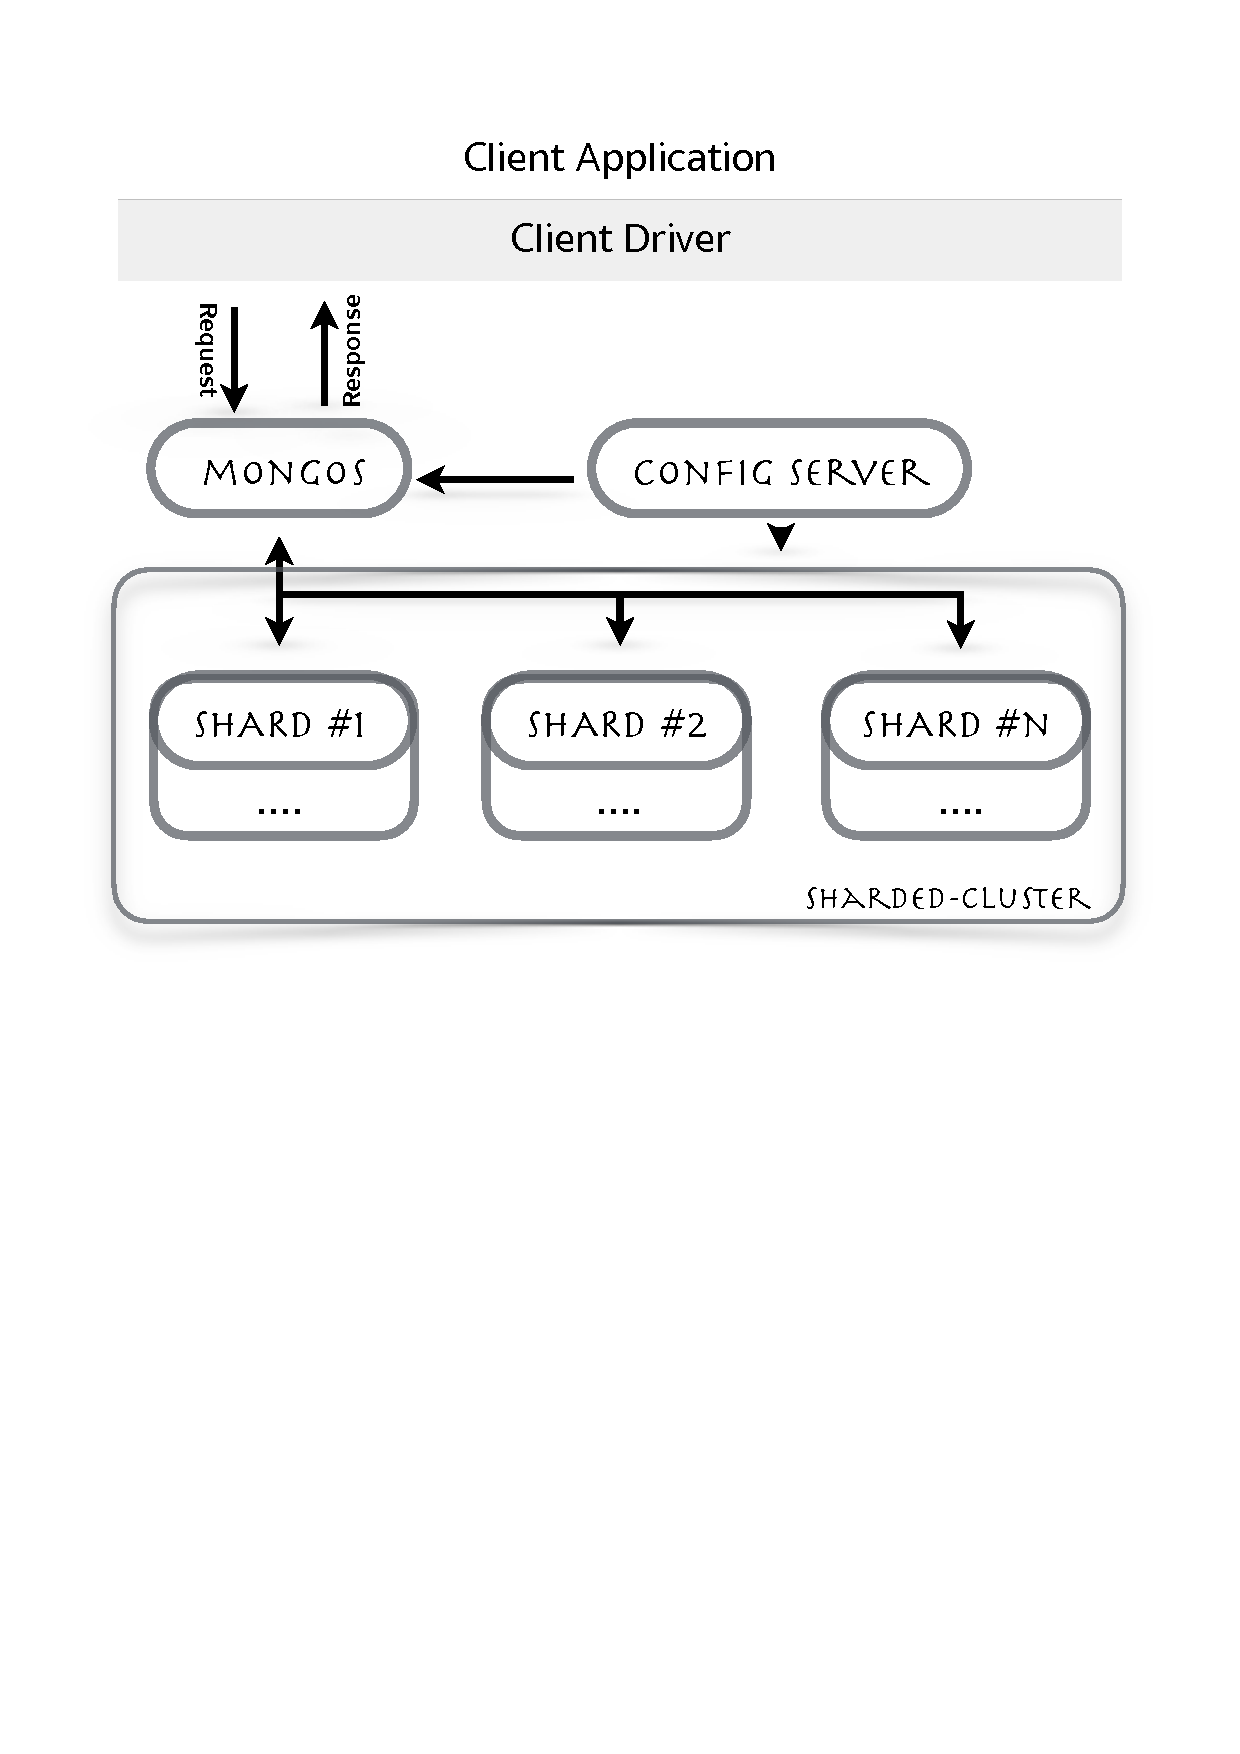
\includegraphics[trim = 0mm 139mm 0mm 23mm, clip, width=0.7\textwidth]{resources/replicaSet/shardedCluster}
\caption[Horizontale Skalierung \textit{(Sharding)}]{Horizontale Skalierung \textit{(Sharding)}}
\label{img:shardedCluster}
\end{figure}

Das Ziel des Ganzen ist die horizontale Skalierbarkeit an Datenmengen, um die Performance des Datenbanksystems zu steigern.
\subsection{Replikation (Replication)}\label{replication}
Manchmal kann es dazu kommen, dass ein Server ausfällt und die Schreib- und Lesezugriffe dadurch auf eine kurze Zeit nicht mehr möglich sind. Um Schreib- und Lesezugriffe auch im Fall eines Serverausfalles ständig ermöglichen zu können, hat \mongo\ einen Replikationsmechanismus entwickelt. Der Replikationsmechanismus dient zur Replikation bzw. zum Spiegeln der Daten auf mehreren Servern und funktioniert nach einem \textit{Master-n-Slaves-Prinzip.}
\begin{figure}[H]
   \begin{subfigure}[t]{0.49\textwidth}\vspace{0pt}
   \centering
      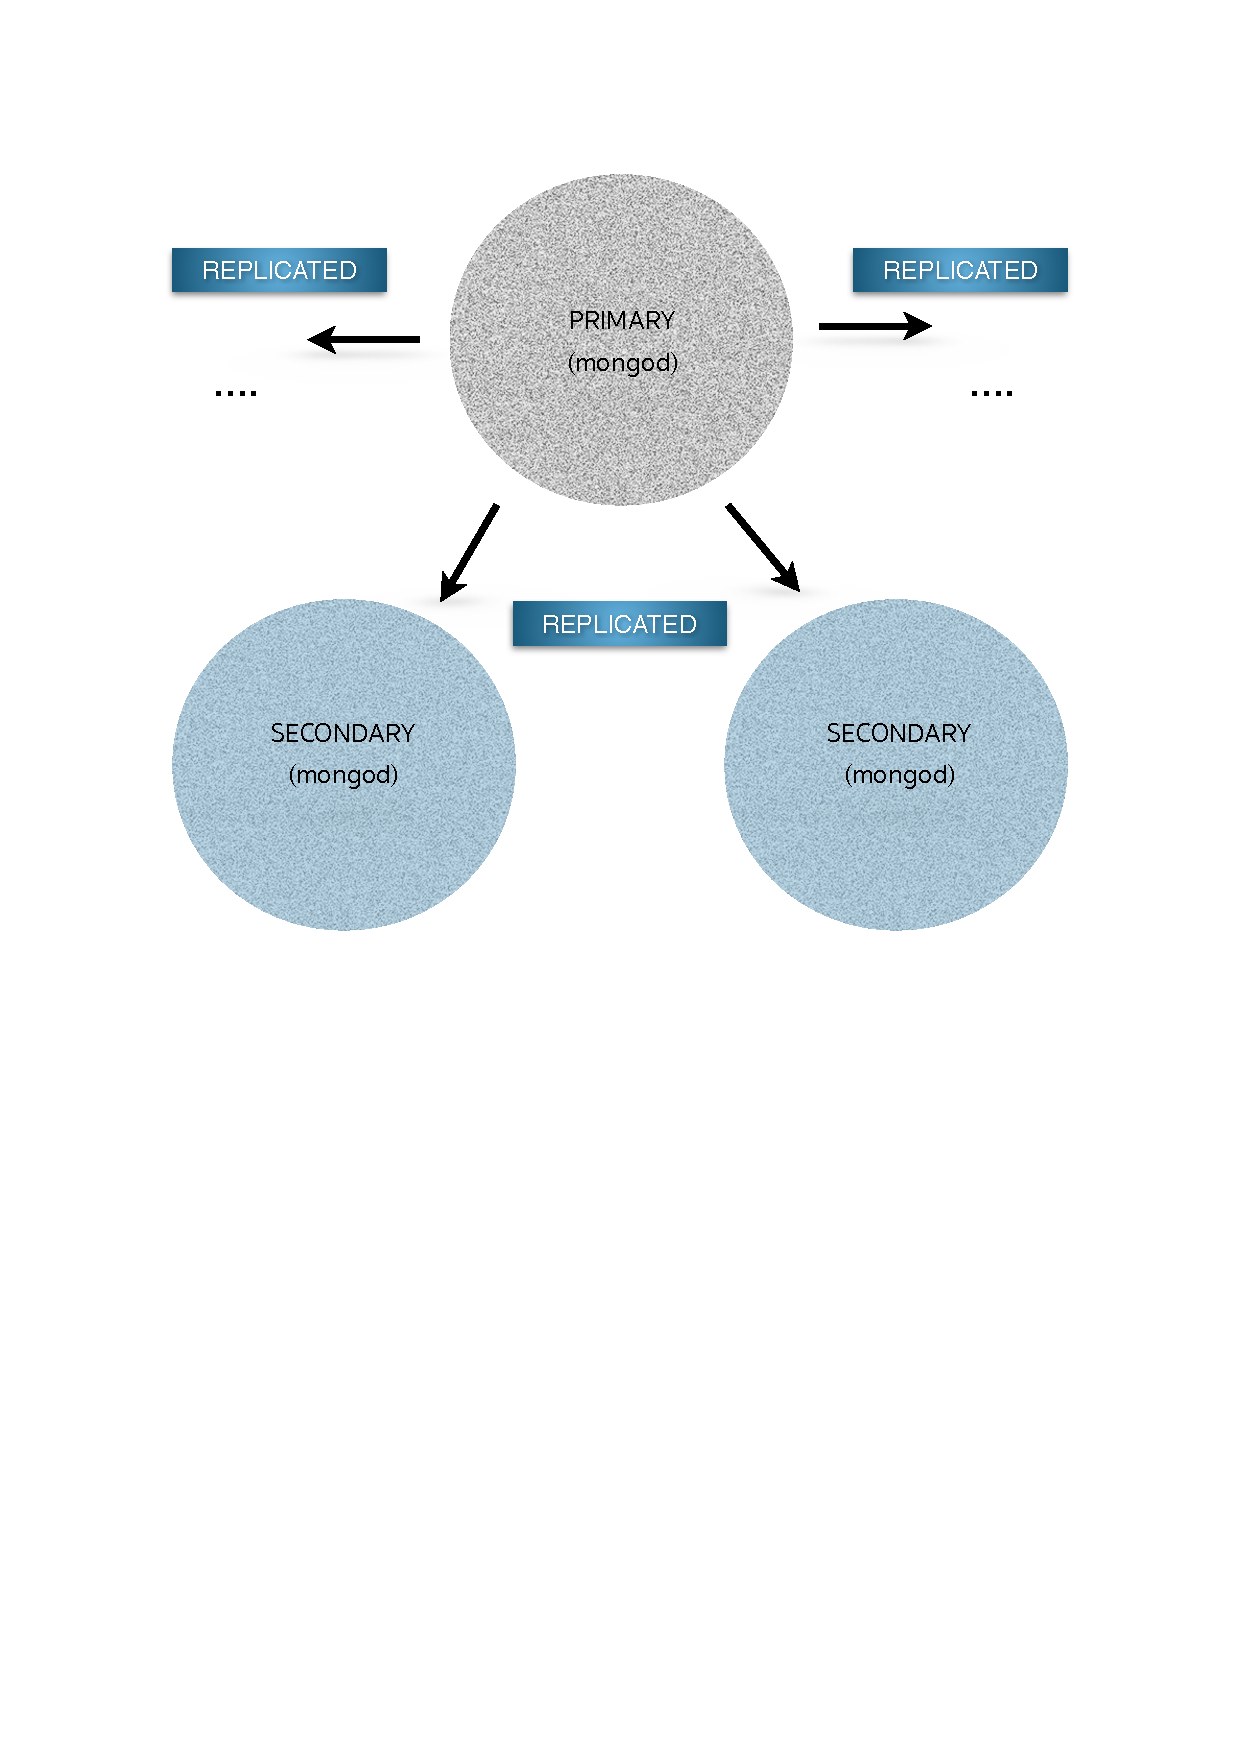
\includegraphics[trim = 28mm 139mm 28mm 29mm, clip, width=0.9\textwidth]{resources/replicaSet/createReplicaSet2}
      \caption[Ein Beispiel für eine Replikationsgruppe]{Ein Beispiel für eine Replikationsgruppe}
      \label{img:createReplicaSet}
   \end{subfigure}\hfill%
   \begin{subfigure}[t]{0.49\textwidth}\vspace{0pt}
   \centering
      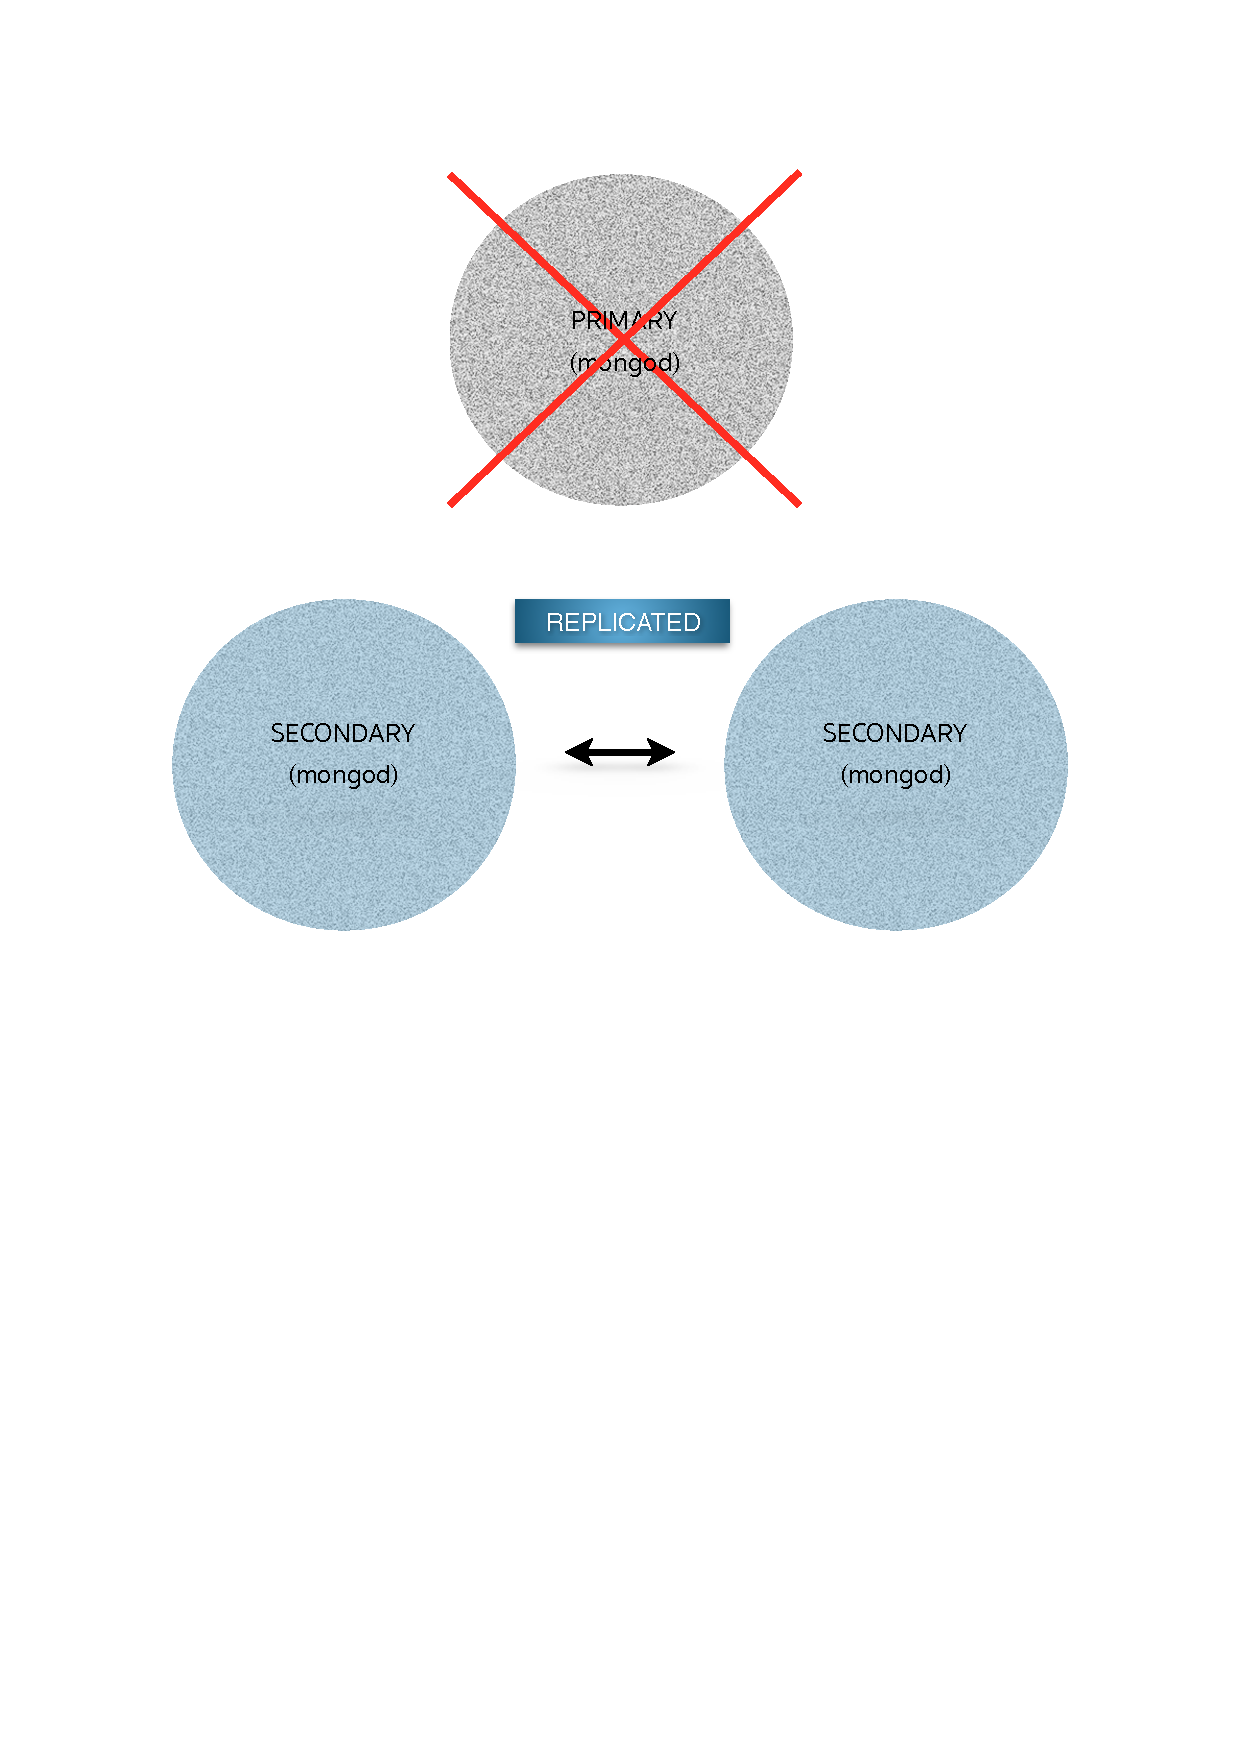
\includegraphics[trim = 28mm 139mm 28mm 29mm, clip, width=0.9\textwidth]{resources/replicaSet/selectNewPrimary}
     \caption[\textbf{Primary} fehlt aus]{\textbf{Primary} fehlt aus}
      \label{img:selectNewPrimary}
   \end{subfigure}\\[5pt]%
   \centering
   \begin{subfigure}[t]{0.49\textwidth}\vspace{0pt}
   \centering
        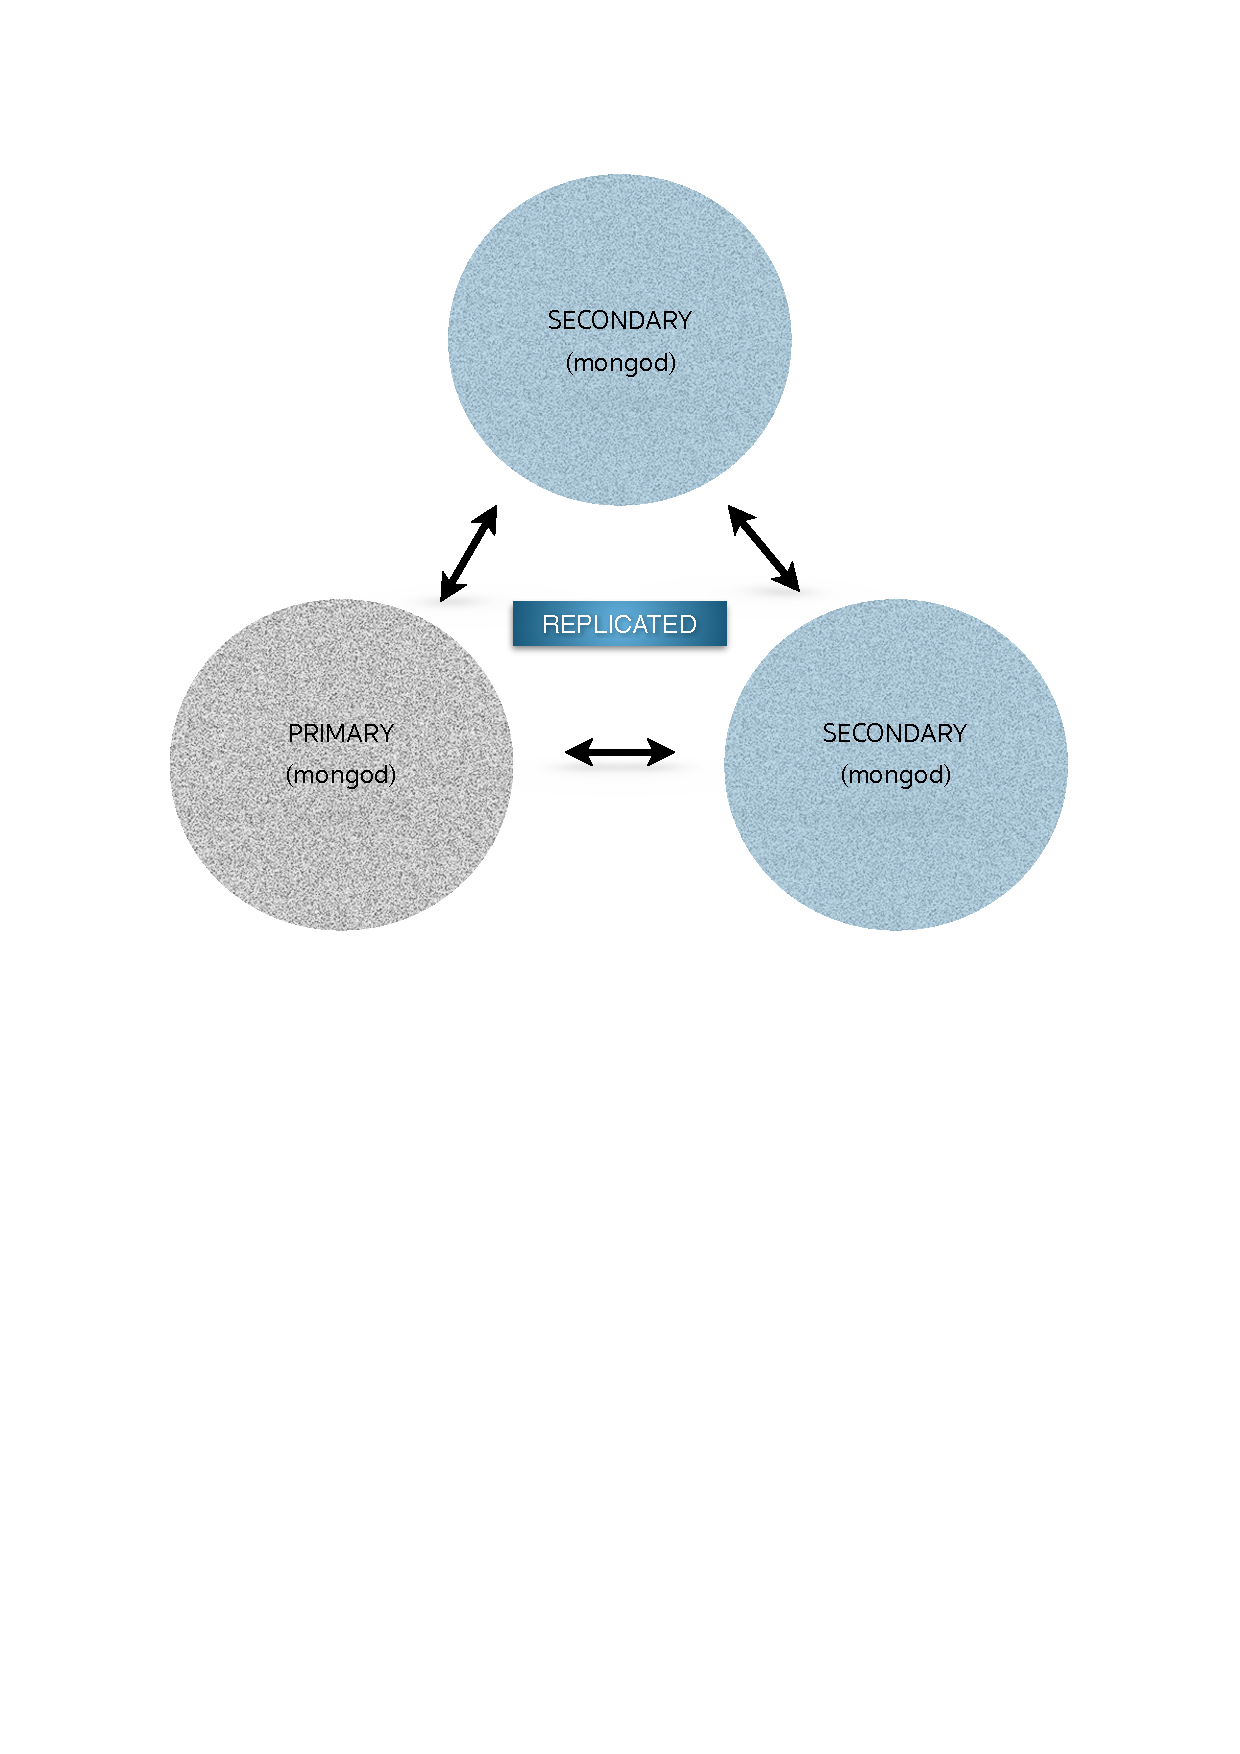
\includegraphics[trim = 28mm 139mm 28mm 29mm, clip, width=0.9\textwidth]{resources/replicaSet/newReplicaSet}
      \caption[Ein neuer \textbf{Primary} wurde gewählt]{Ein neuer \textbf{Primary} wurde gewählt}
      \label{img:newReplicaSet}
   \end{subfigure}
   \caption{Szenario für eine Replikationsgruppe mit drei Servern in einer \textit{Shard}}
   \label{img:replicaSetSzenario}
\end{figure}
Ein \textit{Master}, auch ein \textit{Primary} genannt, besitzt Schreib- und Leserechte. Dieser repliziert die Daten auf \textit{n-Slaves}, die auch als \textit{Secondaries} bezeichnet werden. Ein \textit{Primary} mit \textit{n-Secondaries} bilden gemeinsam eine \textit{Shard}. Eine \textit{Shard} kann aus mind. einem Server bestehen. Falls eine \textit{Shard} aus mehreren Servern besteht, so kann \mongo\ die Server in Replikationsgruppe \textit{(Replica set)} anordnen, damit bei Ausfall eines Servers die Verfügbarkeit der Datenbank trotzdem gewährleistet ist. Mit Replikationsgruppen will \mongo\ die Ausfallsicherheit sicherstellen. Die Abbildung \ref{img:replicaSetSzenario} veranschaulicht ein Szenario für eine Replikationsgruppe mit drei Knoten. Jeder Knoten aus der Gruppe ist als einen eigenen Server vorzustellen. Das \textit{Master-n-Slaves-Prinzip} besagt, dass in einer Replikationsgruppe nur ein Master und n-Slaves existieren können, um eine strenge Konsistenz gewährleisten zu können. 
%\begin{figure}[H]
%\centering
%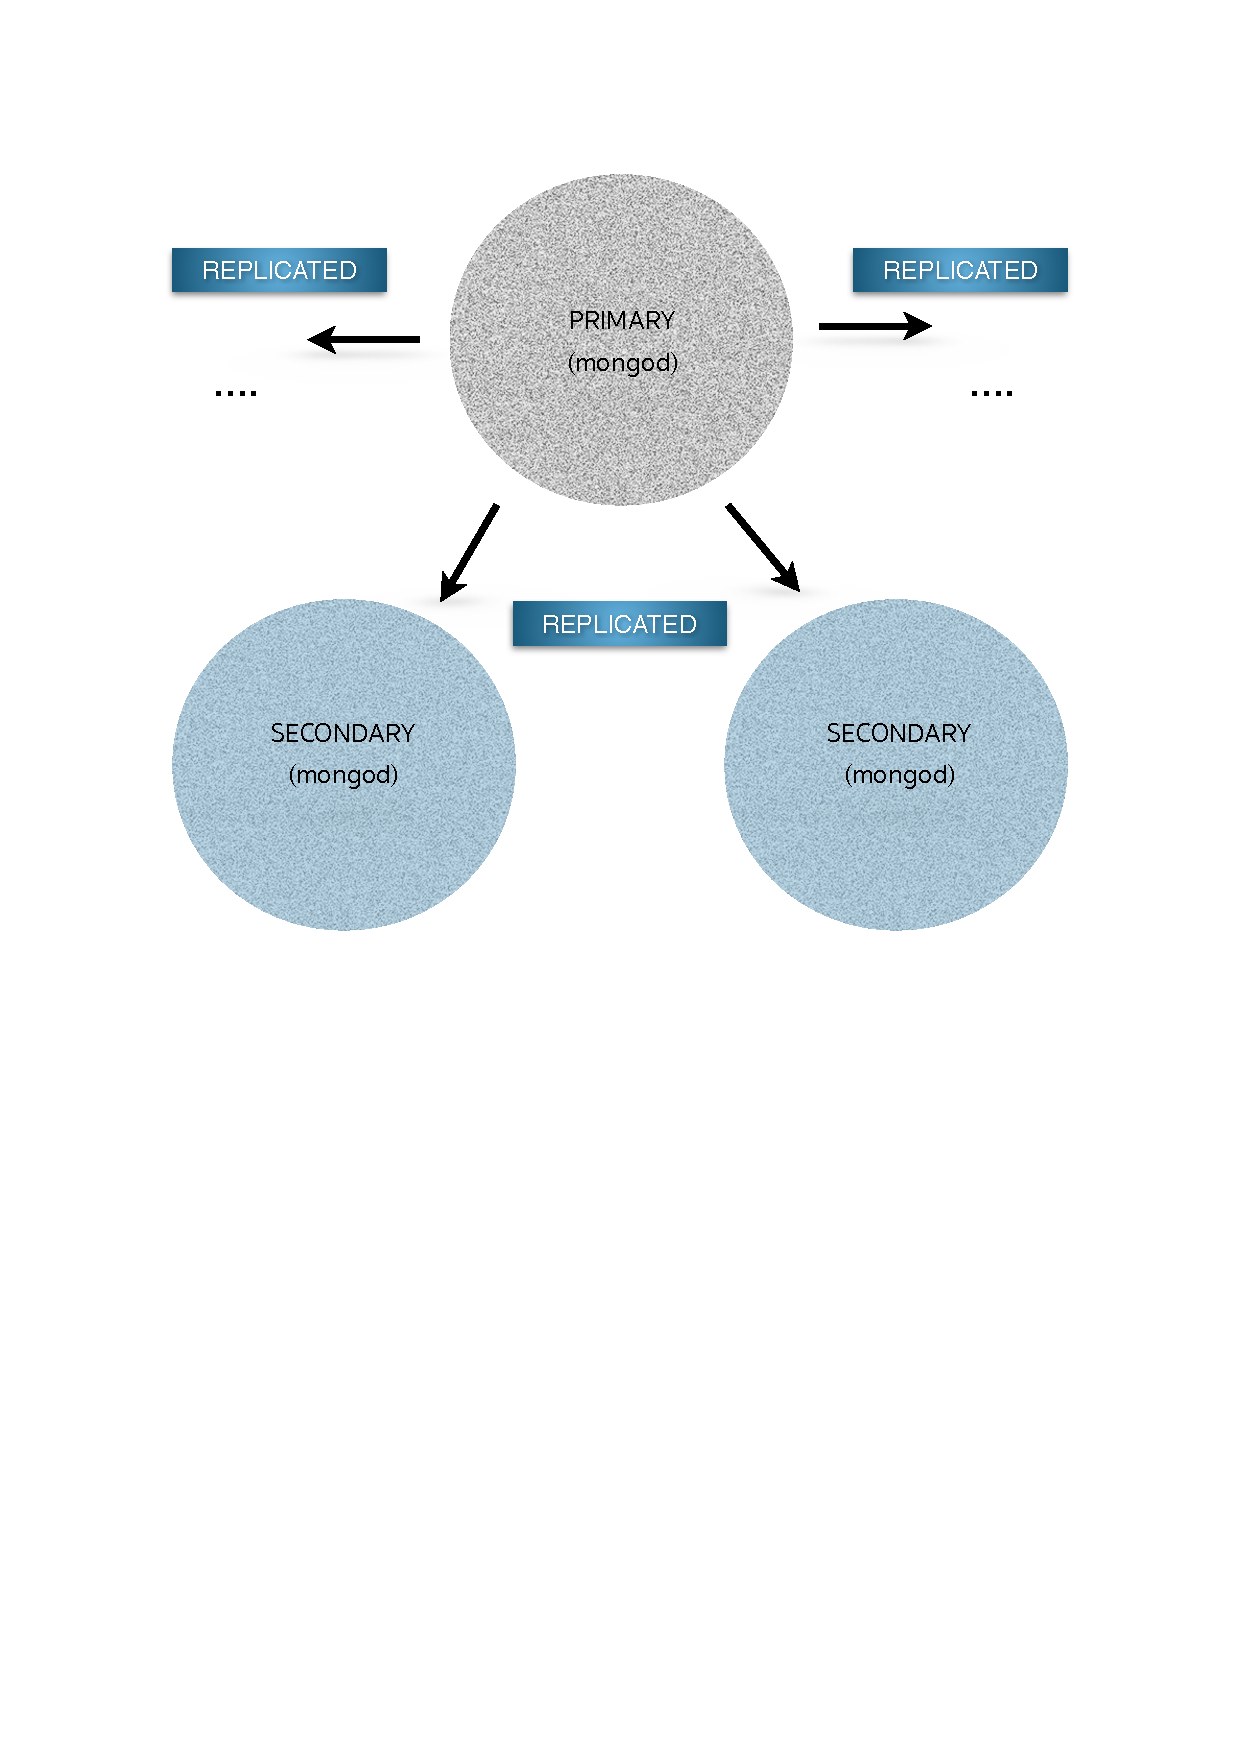
\includegraphics[trim = 0mm 139mm 0mm 28mm, clip, width=0.7\textwidth]{resources/replicaSet/createReplicaSet2}
%\caption[Ein Beispiel für eine Replikationsgruppe]{Ein Beispiel für eine Replikationsgruppe}
%\label{img:createReplicaSet}
%\end{figure}

%\begin{figure}[H]
%\centering
%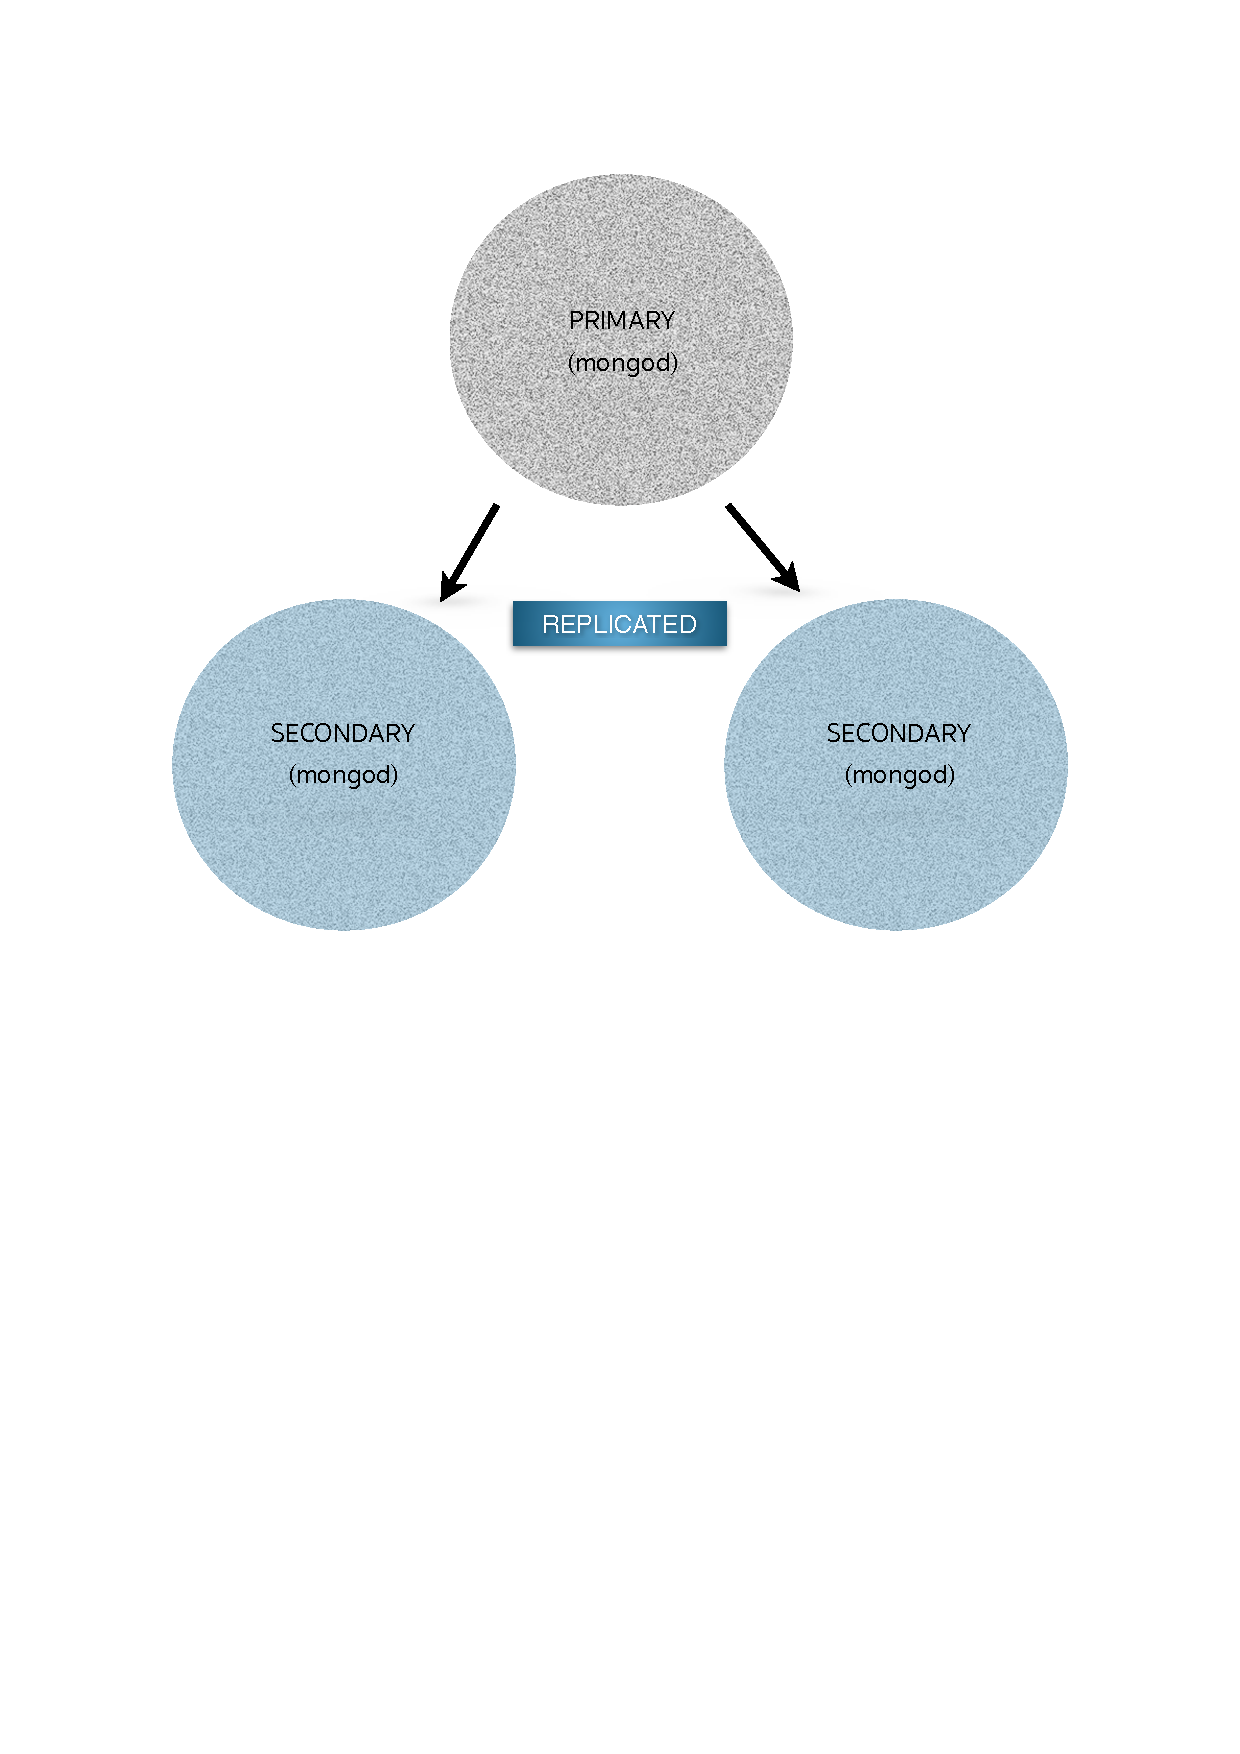
\includegraphics[trim = 0mm 139mm 0mm 9mm, clip, width=0.7\textwidth]{resources/replicaSet/createReplicaSet}
%\caption[Eine Replikationsgruppe mit einem Master und n-Slaves erzeugen]{Eine Replikationsgruppe mit einem Master und n-Slaves erzeugen}
%\label{img:createReplicaSet}
%\end{figure}
\begin{figure}[H]
   \begin{subfigure}[t]{0.49\textwidth}\vspace{0pt}
   \centering
    	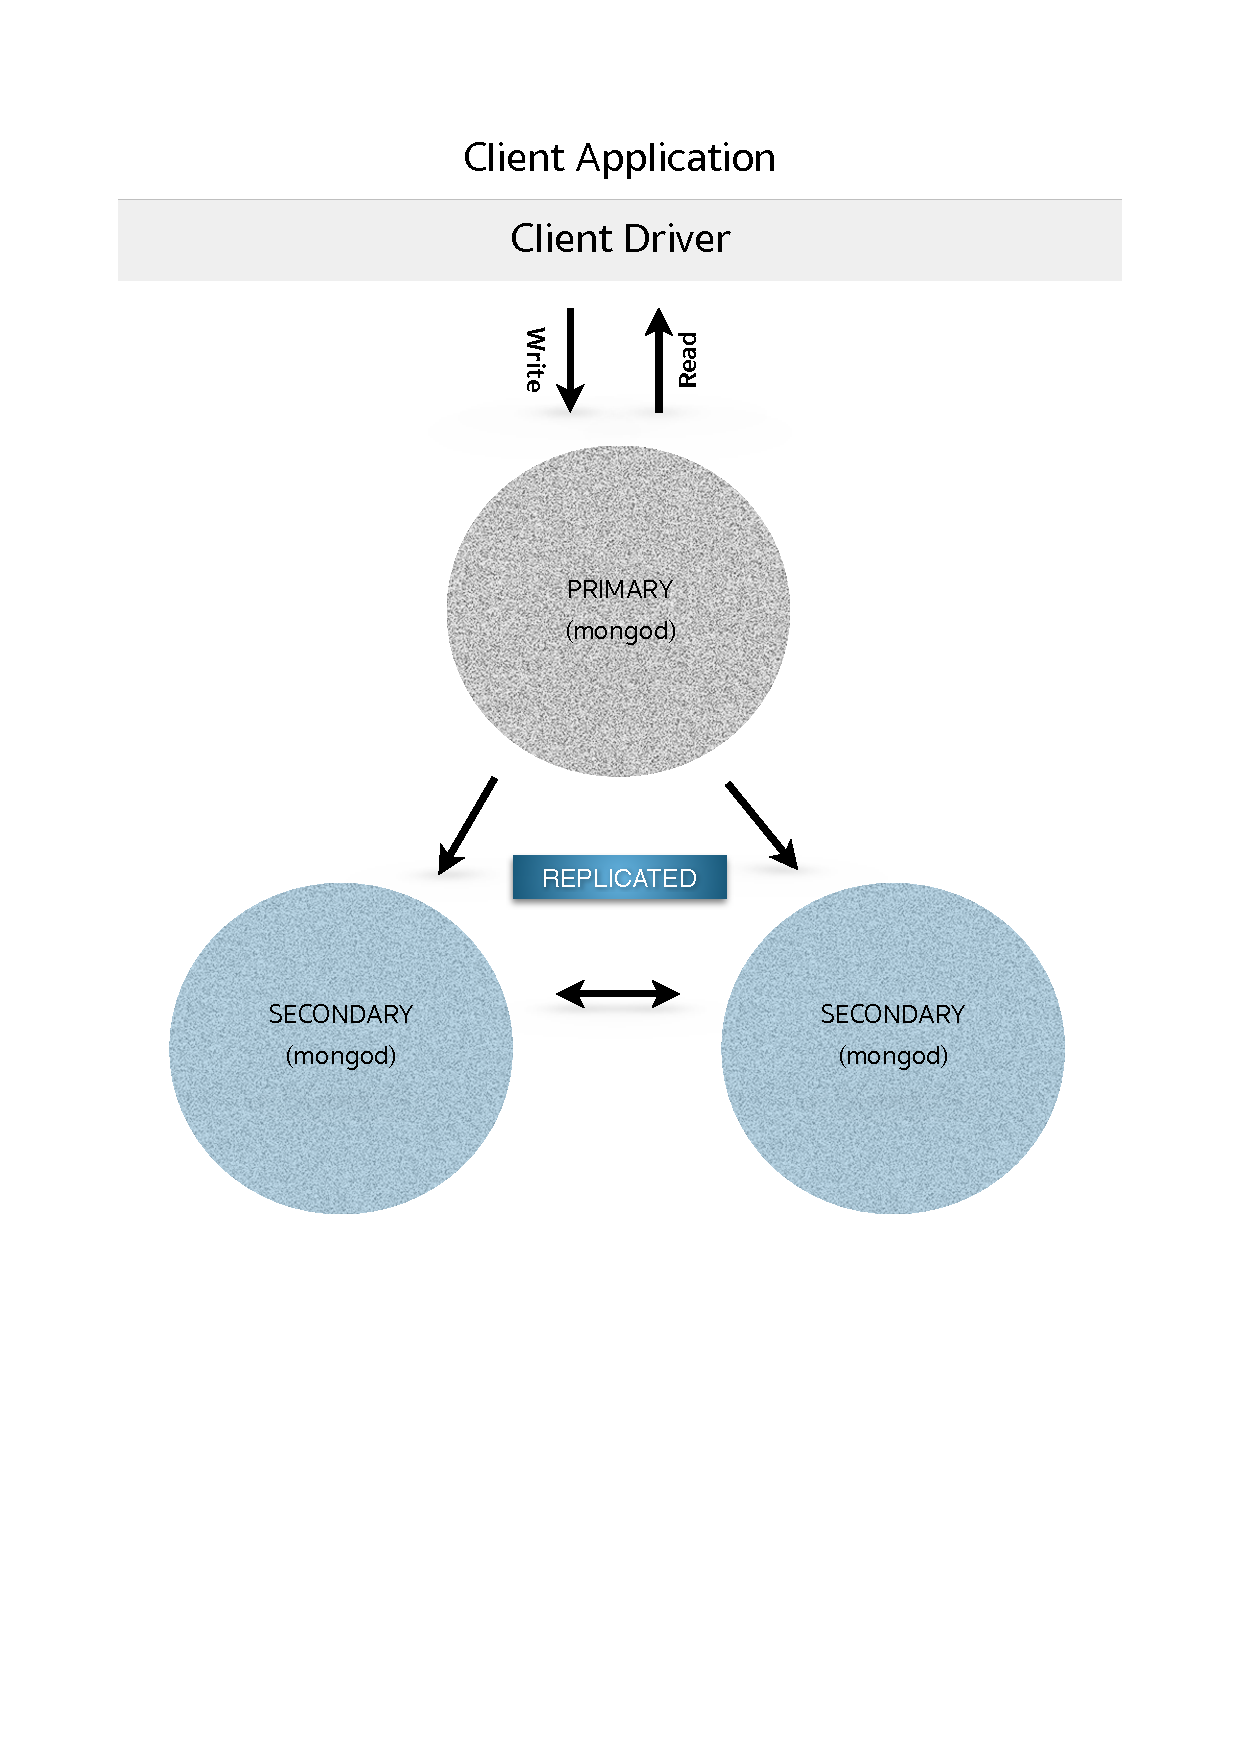
\includegraphics[trim = 0mm 90mm 0mm 20mm, clip, width=1.0\textwidth]{resources/replicaSet/replicaSetStrongConsistency}
	\caption[Lesezugriffe nur über Primary möglich]{Lesezugriffe nur über \textbf{Primary} möglich}
	\label{img:slaveNotOk}
   \end{subfigure}\hfill%
   \begin{subfigure}[t]{0.49\textwidth}\vspace{0pt}
   \centering
	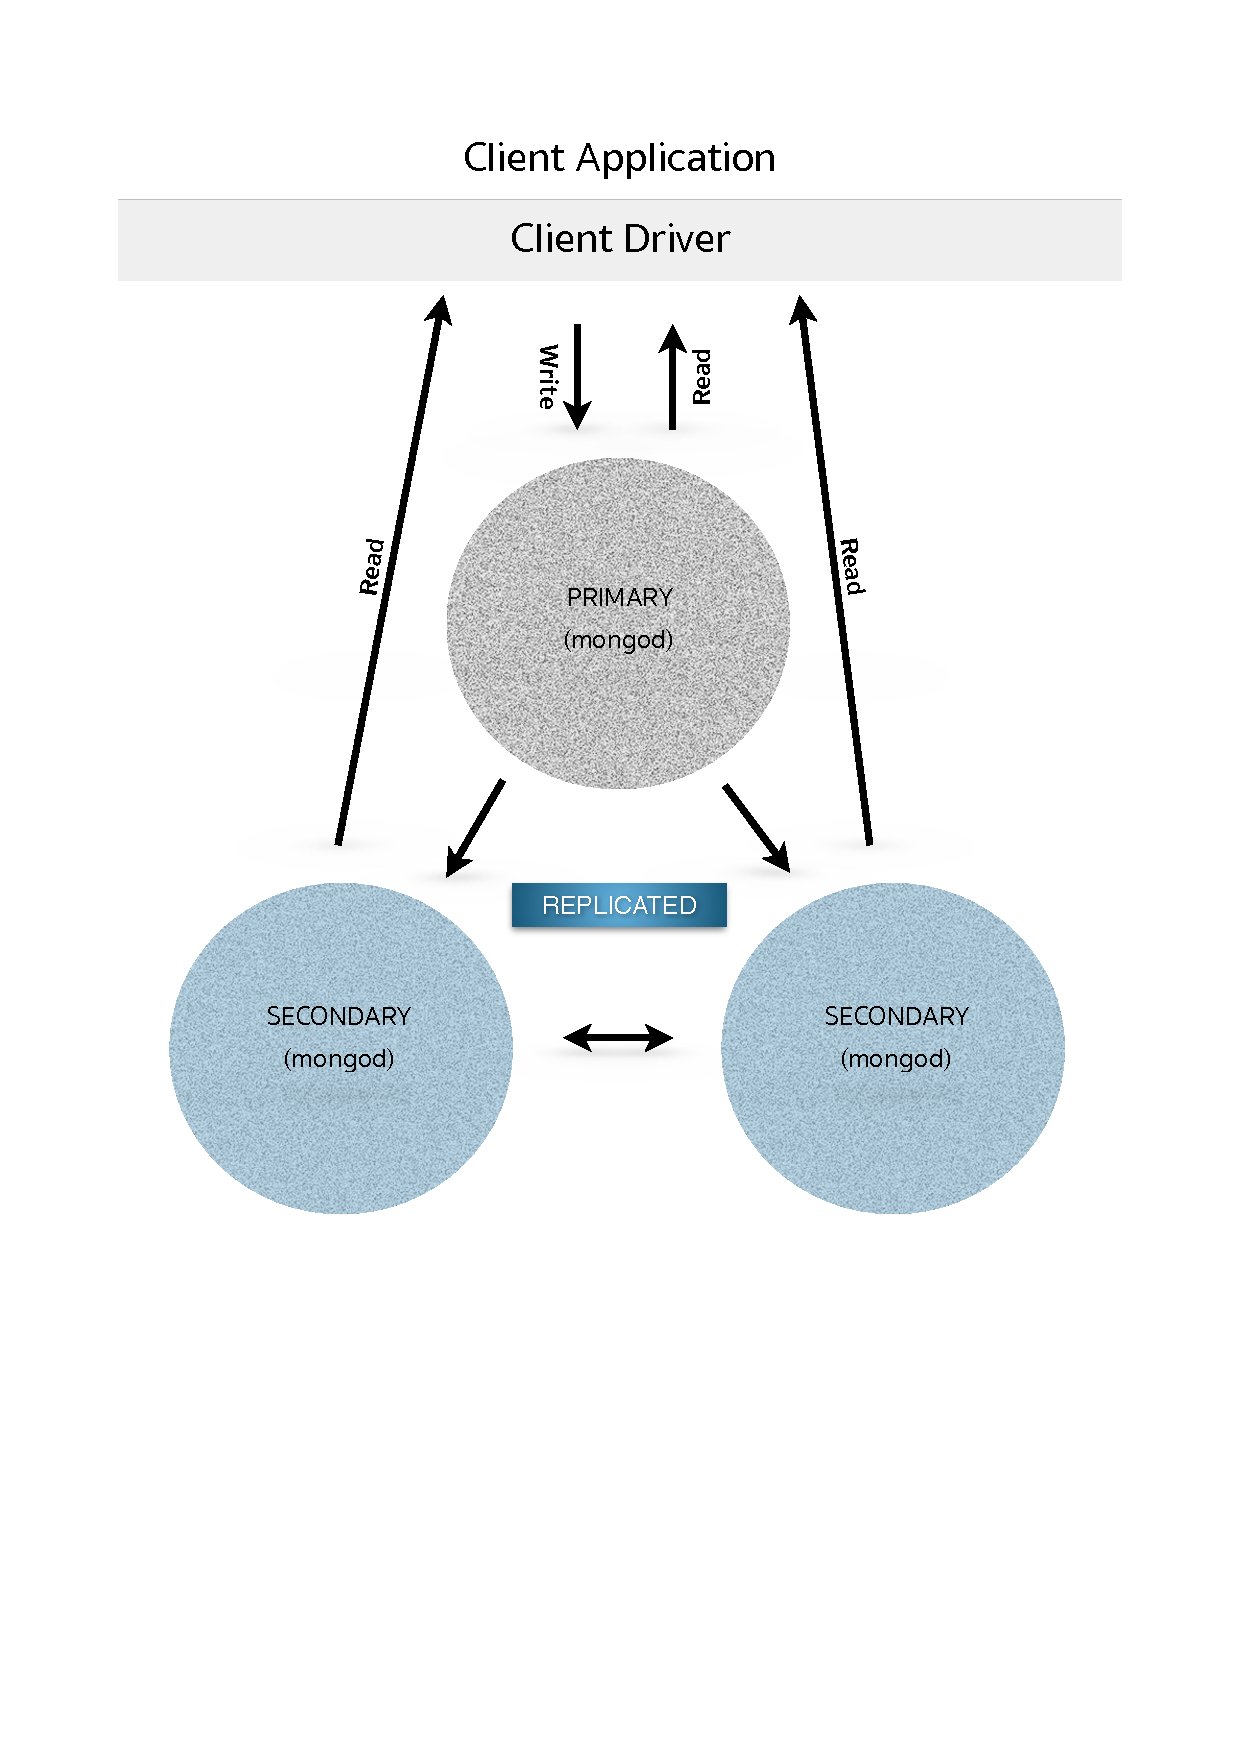
\includegraphics[trim = 0mm 90mm 0mm 20mm, clip, width=1.0\textwidth]{resources/replicaSet/eventualConsistency}
	\caption[Lesezugriffe auch über Secondaries freigeschaltet]{Lesezugriffe auch über \textbf{Secondaries} freigeschaltet}
	\label{img:slaveOk}
   \end{subfigure}\\[5pt]%
   \caption{Freischaltung der Lesezugriffe}
   \label{img:secondariesLowToRead}
\end{figure}
Im Gegenteil zu dem Primary sind bei Secondaries die Schreib- und Leserechte von Anfang an nicht möglich. Falls der Kontext der Anwendung verlangt, können nur die Leserechte entsprechend freigeschaltet werden. 
%\begin{figure}[H]
%\centering
%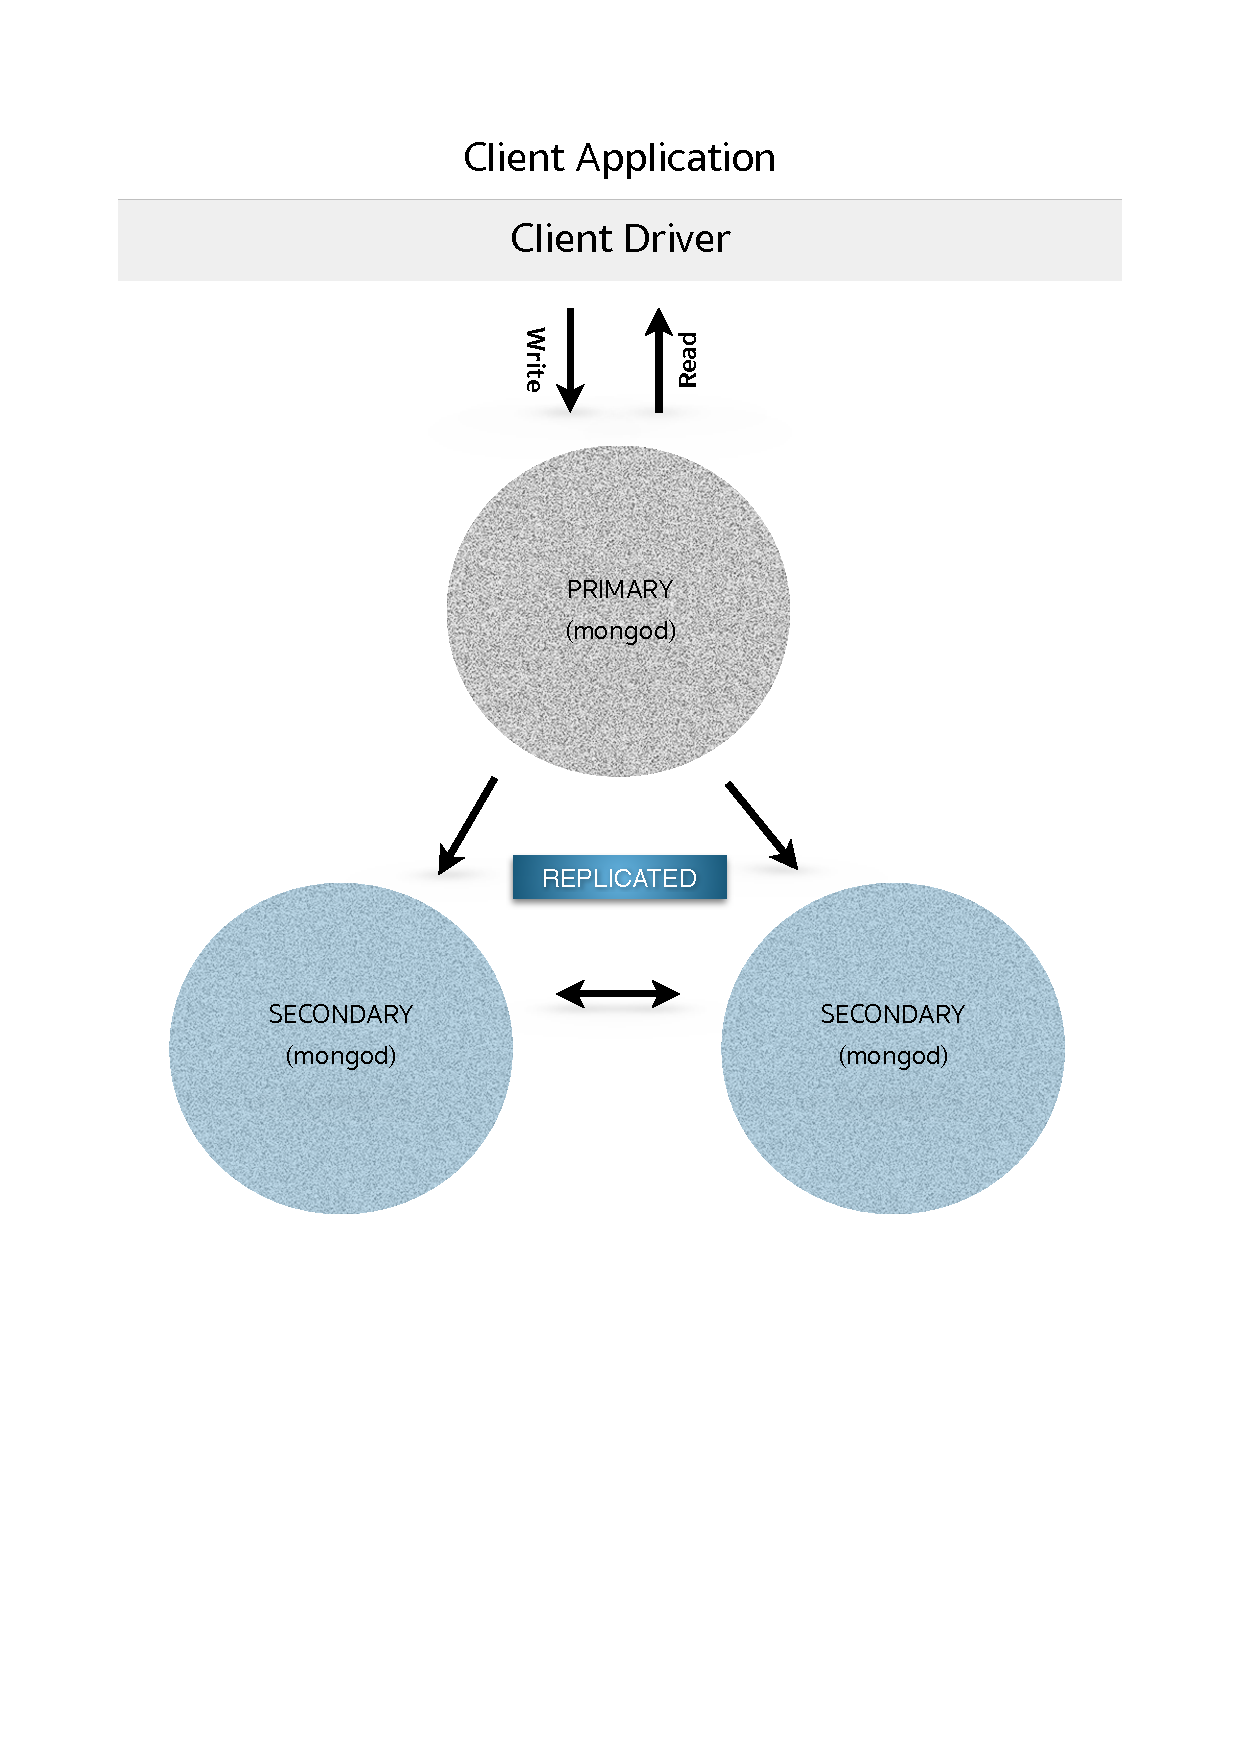
\includegraphics[trim = 0mm 90mm 0mm 20mm, clip, width=0.7\textwidth]{resources/replicaSet/replicaSetStrongConsistency}
%\caption[Lesezugriffe nur über Primary möglich]{Lesezugriffe nur über \textbf{Primary} möglich}
%\label{img:slaveNotOk}
%\end{figure}
%
%\begin{figure}[H]
%\centering
%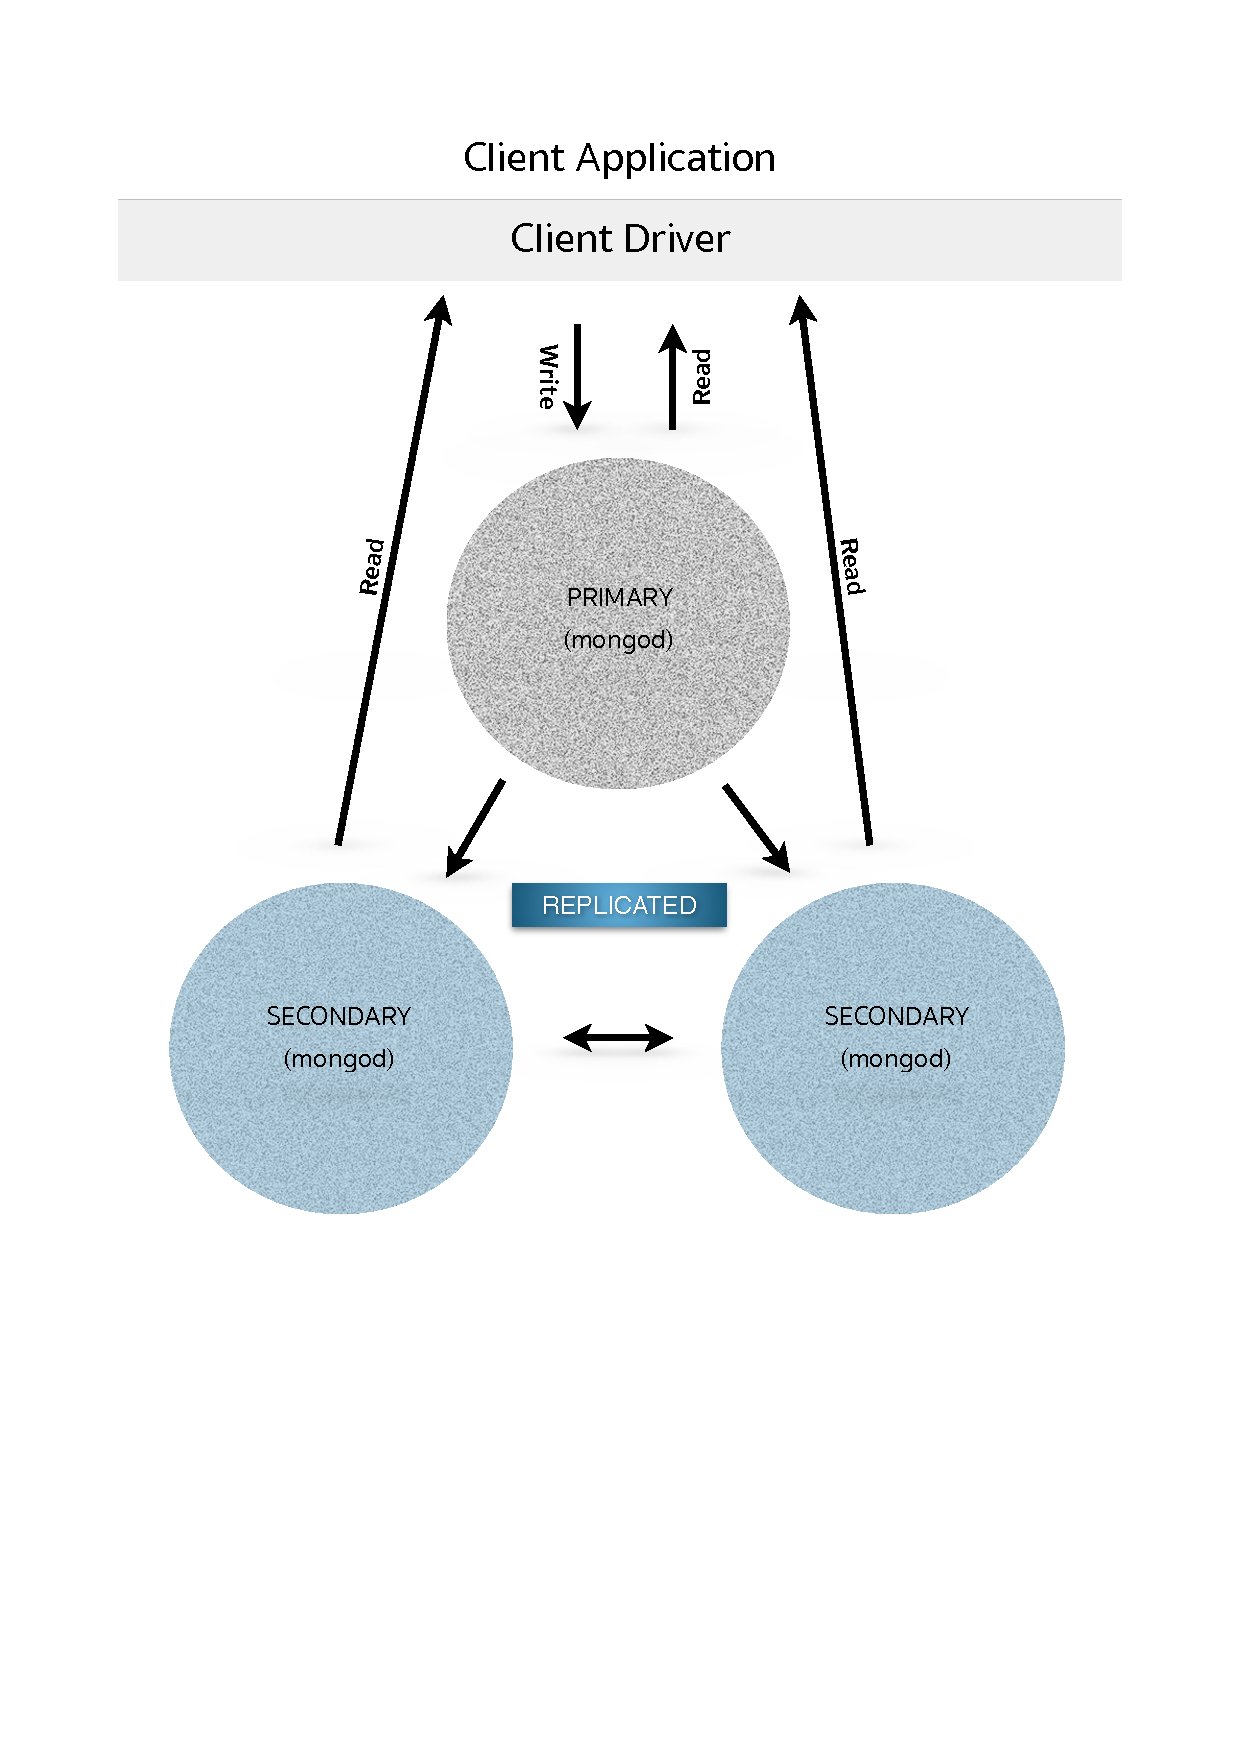
\includegraphics[trim = 0mm 90mm 0mm 20mm, clip, width=0.7\textwidth]{resources/replicaSet/eventualConsistency}
%\caption[Lesezugriffe auch über Secondaries freigeschaltet]{Lesezugriffe auch über \textbf{Secondaries} freigeschaltet}
%\label{img:slaveOk}
%\end{figure}

%\begin{figure}[H]
%\centering
%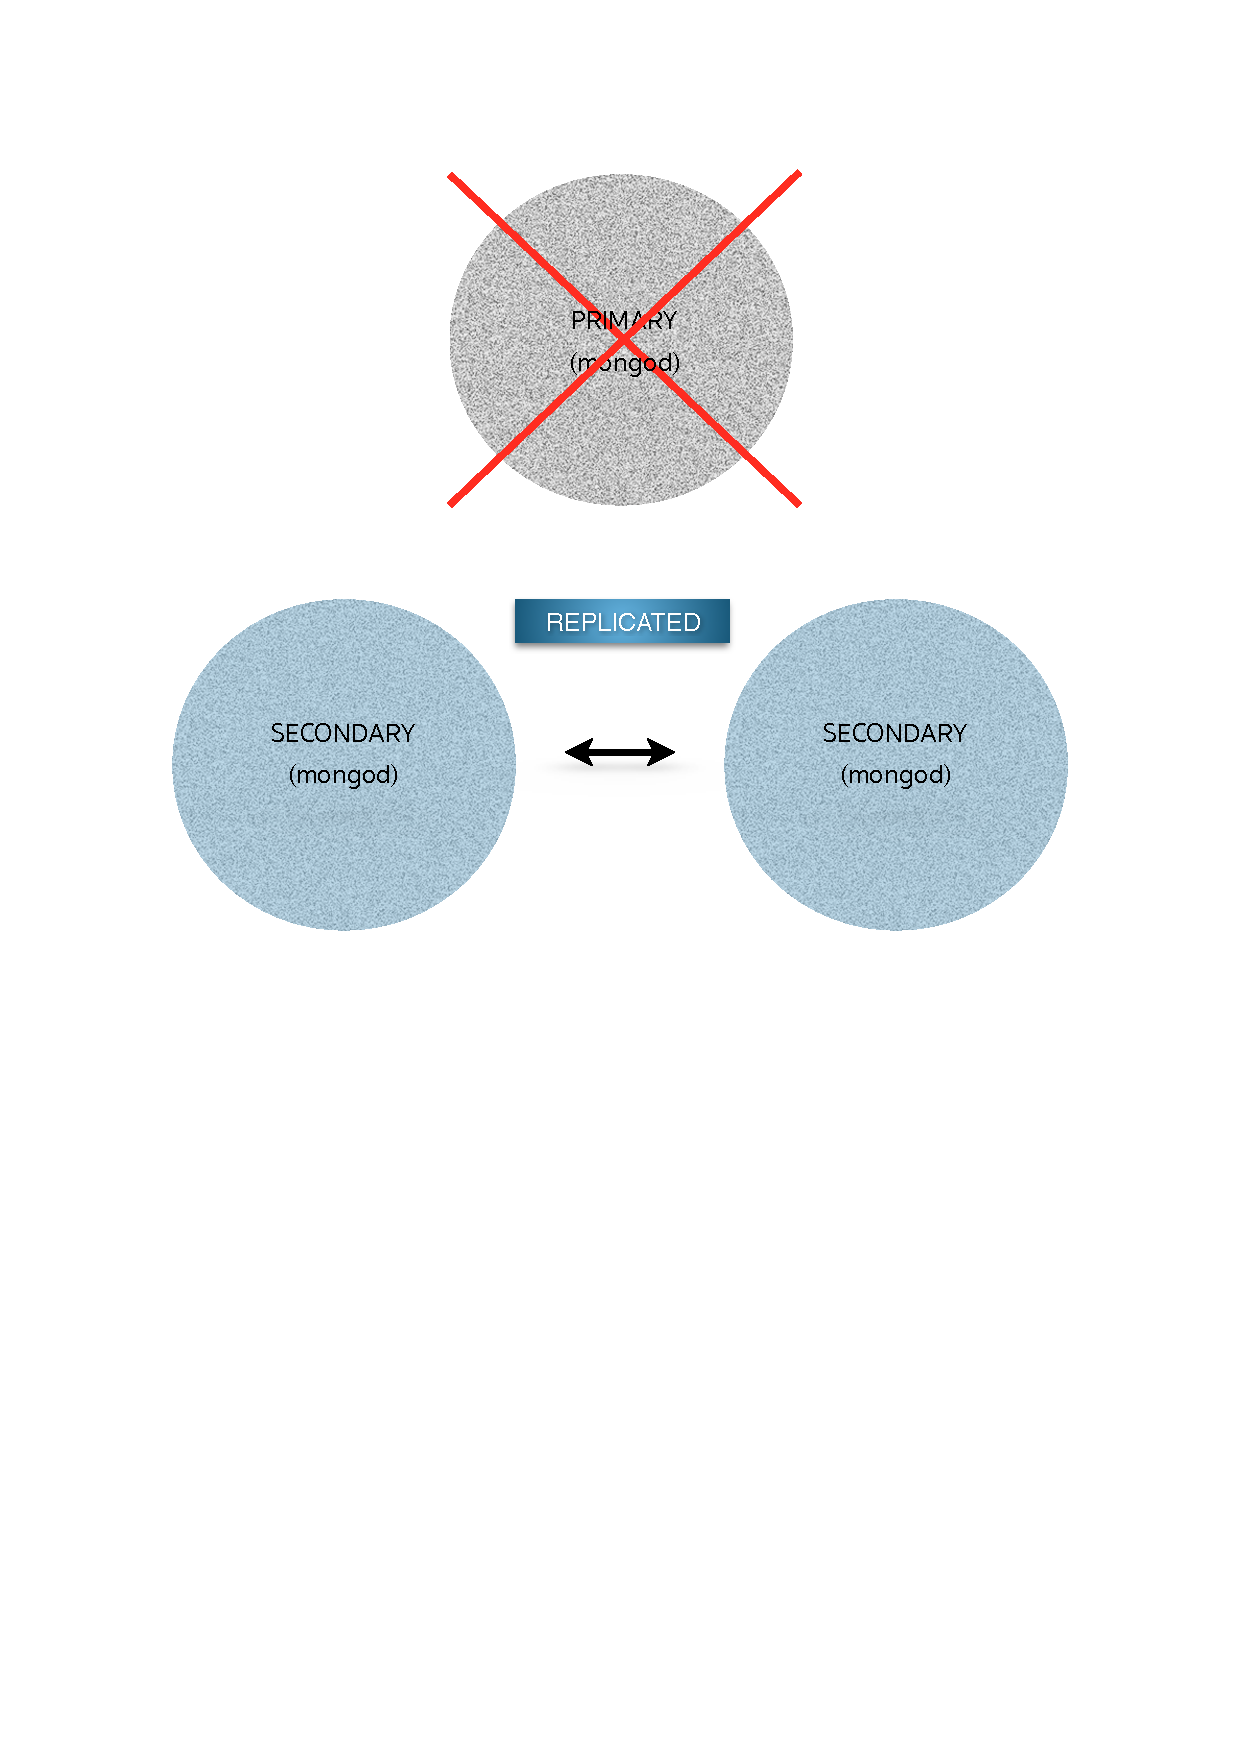
\includegraphics[trim = 0mm 139mm 0mm 28mm, clip, width=0.7\textwidth]{resources/replicaSet/selectNewPrimary}
%\caption[\textbf{Primary} fehlte aus]{\textbf{Primary} fehlte aus}
%\label{img:selectNewPrimary}
%\end{figure}

%\begin{figure}[H]
%\centering
%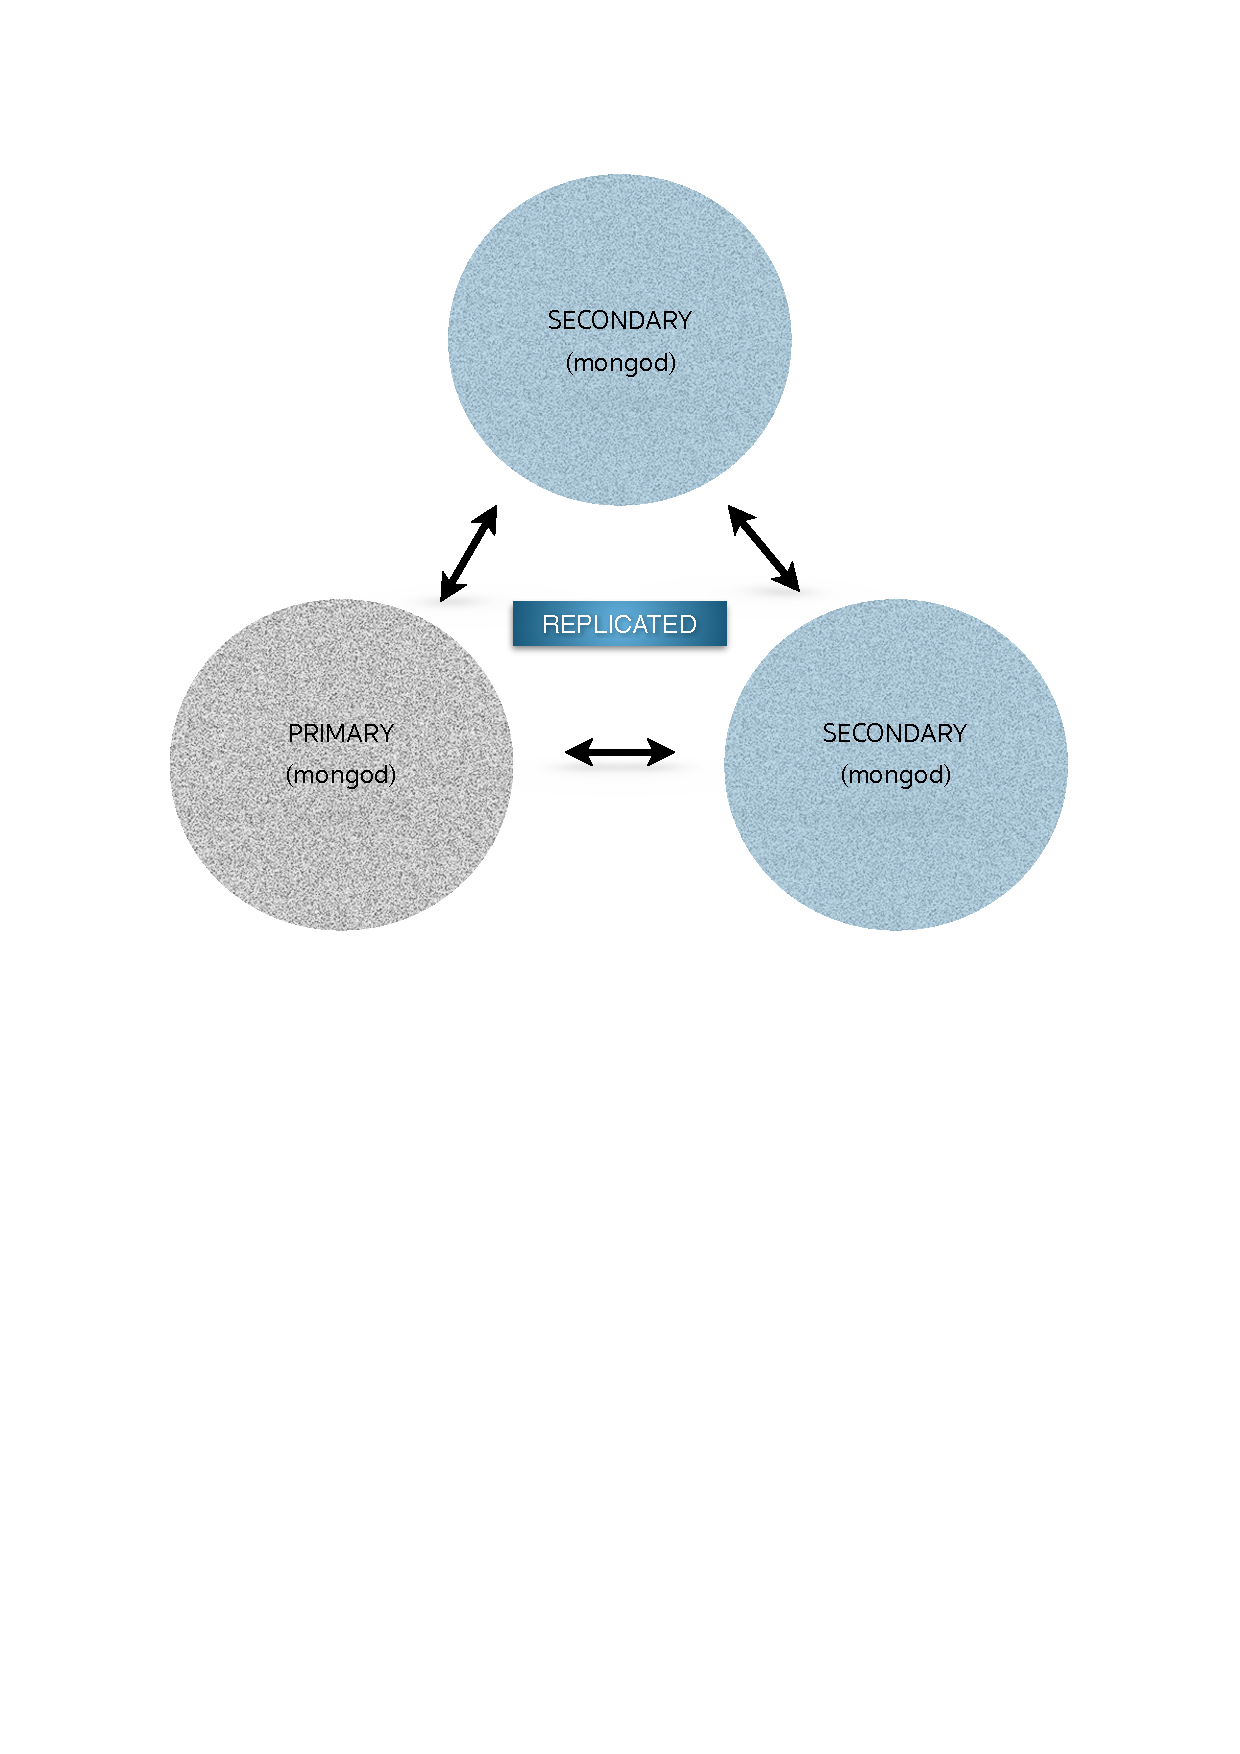
\includegraphics[trim = 0mm 139mm 0mm 28mm, clip, width=0.7\textwidth]{resources/replicaSet/newReplicaSet}
%\caption[Mitglieder der Replikationsgruppe wählten einen neuen \textbf{Primary} aus]{Mitglieder der Replikationsgruppe wählten einen neuen \textbf{Primary} aus}
%\label{img:newReplicaSet}
%\end{figure}
\subsubsection{Eine Replikationsgruppe erzeugen}
In diesem Teilabschnitt wird eine Replikationsgruppe mit insgesamt drei Servern erzeugt. Jeder Schritt der Konfiguration wird in diesem Teilabschnitt nachgespielt.

Um eine Replikationsgruppe effizienter erzeugen zu können, wird ein Skript geschrieben. In dem Skript aus der Abbildung \ref{lst:scriptForCreateOfRep} werden erstmals die Ordner zum Speichern der Daten angelegt. Demnächst ....

\begin{listingsboxShell}[label={lst:scriptForCreateOfRep}]{myshell}{Skript fürs Erstellen einer Replikationsgruppe}
#!/usr/bin/env bash

mkdir -p /data/rs1 /data/rs2 /data/rs3

// Start von drei lokalen mongod-Instanzen als Replikationsgruppe

mongod --replSet m101 --logpath "1.log" --dbpath /data/rs1 --port 27017
--oplogSize 64 --fork --smallfiles
mongod --replSet m101 --logpath "2.log" --dbpath /data/rs2 --port 27018
--oplogSize 64 --smallfiles --fork
mongod --replSet m101 --logpath "3.log" --dbpath /data/rs3 --port 27019
--oplogSize 64 --smallfiles --fork
\end{listingsboxShell}

Das Skript mit dem Inhalt aus Listing \ref{lst:scriptForCreateOfRep} ist mit dem aus Listing \ref{lst:runOfscriptForCreateOfRep} auszuführen:

\begin{listingsboxShell}[label={lst:runOfscriptForCreateOfRep}]{myshell}{Erstellen einer Replikationsgruppe anhand eines Skriptes}
vlfa:scripts vlfa$ bash < create_replica_set.sh
\end{listingsboxShell}

Bei der Ausführung des Skriptes kann zu den Problemen führen. Um aktuelle Prozesse mit mongo anschauen und stoppen zu können, muss man folgenden Befehl angeben. The problem was that I have runned mongod without any parameters before I started launching the nodes. First kill all the mongo, mongod and mongos instances to guarantee the environment is clear.\url{http://stackoverflow.com/questions/25839559/mongodb-server-is-not-running-with-replset}

Find the mongodb process PID by typing: lsof -i:27017 assuming your mongodb is running on port 27017
Type kill <PID>, replace <PID> by the value you found the previous command.

\begin{listingsboxShell}[label={lst:listOfPIDs}]{myshell}{Auflistung aktueller mongo(s,d)-Prozesse}
vlfa:scripts vlfa$ ps -ef | grep 'mongo'

oder besser mit 

lsof -i:27017
\end{listingsboxShell}

Danach ist wichtig, Prozesse zu stoppen. Dafür muss man nach dem Befehl kill die ProzessID eingeben, siehe Listing \ref{lst:killPID}. Dann wird die Möglichkeit fürs Erstellen eigener Replikationsgruppe ermöglicht, siehe dazu Listings \ref{lst:scriptForCreateOfRep} und \ref{lst:runOfscriptForCreateOfRep}.

\begin{listingsboxShell}[label={lst:killPID}]{myshell}{mongo(s,d)-Server zwingend stoppen}
// konkreten mongo(s,d)-Server zwingend stoppen
vlfa:scripts vlfa$ kill 'PID'

// alle mongo(s,d)-Server zwingend stoppen
vlfa:scripts vlfa$ killall mongo(s,d)
\end{listingsboxShell}

Damit ist die Konfigurationsgruppe mit 3 Servern angelegt. Zum Anschauen einer log-Datei;

\begin{listingsboxShell}[label={lst:X}]{myshell}{1.log-Inhalt}
2016-12-19T14:58:11.637+0100 I CONTROL  [initandlisten] MongoDB starting :
pid=25626 port=27017 dbpath=/data/rs1 64-bit host=vlfa.fritz.box
// irrelevant
2016-12-19T14:58:11.639+0100 I CONTROL  [initandlisten] options:
{ net: { port: 27017 }, processManagement: { fork: true }, replication:
{ oplogSizeMB: 64, replSet: "m101" }, storage: { dbPath: "/data/rs1",
mmapv1: {smallFiles: true}}, systemLog: {destination: "file", path: "1.log"}}
// irrelevant
\end{listingsboxShell}
Die Replikationsgruppe starten.......blabla
\begin{listingsboxJavaScript}[label={lst:initReplica}]{myJS}{Skript zum Start der Replikationsgruppe}
config = { _id: "m101", members:[
          { _id : 0, host : "localhost:27017", priority:0, slaveDelay:5},
          { _id : 1, host : "localhost:27018"},
          { _id : 2, host : "localhost:27019"} ]
};

rs.initiate(config);
rs.status();
\end{listingsboxJavaScript}

Die Server aus Listing \ref{lst:initReplica} nehmen nun Kontakt miteinander auf, gründen die Gruppe und wählen den Primary-Server aus. Wie im Skript aus Listing 	\ref{lst:initReplica} zu entnehmen ist, kann der Zustand der Replikationsgruppe mit \texttt{rs.status()} geprüft werden. Bei Ausfall des Primary-Servers wählen die Secondaries untereinander entsprechend einen neuen Primary-Server. Damit wird die Ausfallsicherheit des Servers erreicht. Die Mindestanzahl an Server in einer Replikationsgruppe liegt bei drei. 

\begin{listingsboxShell}[label={lst:runOfInitReplica}]{myshell}{Skript ausführen}
vlfa:scripts vlfa$ mongo --port 27018 < init_replica.js
\end{listingsboxShell}

Die Priorität '0' teilt mit, wer Primary Member in der Replikationsgruppe ist. Korrigieren, Stimmt nicht....\url{https://docs.mongodb.com/v3.2/core/replica-set-priority-0-member/}

\subsection{MongoDB mit Java}

\begin{listingsboxJava}[label={lst:conn}]{myJava}{Verbindungsaufbau}
public static void main(String[] args) {

	MongoClient mongoClient = new MongoClient("localhost", 27017);
        MongoDatabase db = mongoClient.getDatabase("test");
        MongoCollection<Document> collectionOfZips = db.getCollection("zips");
        
        // weitere CRUD-Operationen mit der ausgewählten Kollektion
}
\end{listingsboxJava}

\begin{listingsboxJava}[label={lst:X}]{myJava}{Skript zur Initialisierung der Replikationsgruppe}
public static void main (String[] args) throws InterruptedException {
        MongoClient client = new MongoClient(asList(
                new ServerAddress("localhost", 27017),
                new ServerAddress("localhost", 27018),
                new ServerAddress("localhost", 27019)));
                
                // weitere CRUD-Operationen
}
\end{listingsboxJava}

\begin{listingsboxShell}[label={lst:X}]{myshell}{Simulation des Server-Ausfalls 'PRIMARY'}
m101:PRIMARY> rs.stepDown()

Result:

2016-12-19T21:24:12.739+0100 I NETWORK  [thread1]
trying reconnect to 127.0.0.1:27018 (127.0.0.1) failed
2016-12-19T21:24:12.760+0100 I NETWORK  [thread1]
reconnect 127.0.0.1:27018 (127.0.0.1) ok
m101:SECONDARY> 
\end{listingsboxShell}

Der aktuelle MongoDB Java Treiber ist in Version 3.4.0 verfügbar und kann bequem als Maven Dependency geladen werden, siehe Listing  \ref{lst:mongoJDriver}.
 
\begin{listingsboxJava}[label={lst:mongoJDriver}]{myxml}{MongoDB Java Treiber in Version 3.4.0 als Maven Dependency}
<dependency>
        <groupId>org.mongodb</groupId>
        <artifactId>mongo-java-driver</artifactId>
        <version>3.4.0</version>
</dependency>
\end{listingsboxJava}

Um die Sicherung der Zugehörigkeit der Mitglieder zu konkreter Replikationsgruppe festzustellen, siehe Listing \ref{lst:guarantee}, Zeilen 6-8...
\begin{listingsboxJava}[label={lst:guarantee}]{myJava}{Sicherung der Zugehörigkeit zu konkreter Replikationsgruppe}
 public static void main (String[] args) throws InterruptedException {
        MongoClient client = new MongoClient(asList(
                new ServerAddress("localhost", 27017),
                new ServerAddress("localhost", 27018),
                new ServerAddress("localhost", 27019)), 
                MongoClientOptions.builder()
                        .requiredReplicaSetName("m101")
                        .build());
\end{listingsboxJava}


%\section{Apache Cassandra}
%Cassandra\footnote{Apache Cassandra: \url{http://cassandra.apache.org}, zugegriffen am 16. Dezember 2016} zählt, neben MongoDB\footnote{MongoDB: \url{https://www.mongodb.com}, zugegriffen am 16. Dezember 2016}, zu den derzeit populärsten NoSQL-Datenbanken. Cassandra war ursprünglich eine proprietäre Datenbank von Facebook und wurde 2008 als Open-Source-Datenbank veröffentlicht. Beispiele für weitere NoSQL-Datenbanken sind SimpleDB\footnote{SimpleDB: \url{https://aws.amazon.com/de/simpledb/}, zugegriffen am 16. Dezember 2016}, Google Big Table\footnote{Google Big Table: \url{https://research.google.com/archive/bigtable.html}, zugegriffen am 16. Dezember 2016}, Apache Hadoop\footnote{Apache Hadoop: \url{http://hadoop.apache.org}, zugegriffen am 16. Dezember 2016}, MapReduce\footnote{MapReduce: \url{http://hortonworks.com/apache/mapreduce/}, zugegriffen am 16. Dezember 2016}, MemcacheDB\footnote{MemcacheDB: \url{http://memcachedb.org}, zugegriffen am 16. Dezember 2016} und Voldemort\footnote{Voldemort: \url{http://www.project-voldemort.com/voldemort/}, zugegriffen am 16. Dezember 2016}. Unternehmen, die auf NoSQL setzen, sind unter anderem NetFlix\footnote{NetFlix: \url{https://www.netflix.com/de-en/}}, LinkedIn\footnote{LinkedIn: \url{https://www.linkedin.com/feed/}} und Twitter\footnote{Twitter: \url{https://twitter.com/?lang=en}}.\footnote{NoSQL: \url{http://www.searchenterprisesoftware.de/definition/NoSQL}, zugegriffen am 16. Dezember 2016}\newline
%
%Cassandra ist als skalierbares, ausfallsicheres System für den Umgang mit großen Datenmengen auf verteilten Systemen (Clustern) konzipiert. Sie ist die beliebteste spaltenorientierte NoSQL-Datenbank und im Gegensatz zu MongoDB (C++) in Java geschrieben. Aufgrund ihrer architektonischen Eigenschaften wird Cassandra häufig in Big-Data-Projekten eingesetzt, kann in Zusammenarbeit mit einem Applikations-Server/Framework aber auch gut für komplexe Webanwendungen verwendet werden.
